\chapter {Preparation of Numerical Modeling Framework for Engineering Extreme Storm Analyses}
\label{ch:JHE}
 
This chapter has been published in its current form in the \textit{Journal of Hydrologic Engineering}. \textcopyright American Society of Civil Engineers. Used with permission.\\

\bigbreak

\noindent
\hangafter=1
\setlength{\hangindent}{2em}
Chen, X., Hossain, F., and Leung, R. L. (2017), Establishing a Numerical Modeling Framework for Hydrologic Engineering Analyses of Extreme Storm Events, \textit{Journal of Hydrologic Engineering}, 22(8), 04017016. doi:10.1061/(ASCE)HE.1943-5584.0001523.

\vspace{10mm}

\noindent
\textit{\textbf{Abstract}}
 
In this study a numerical modeling framework for simulating extreme storm events was established using the Weather Research and Forecasting (WRF) model. \
Such a framework is necessary for the derivation of engineering parameters such as probable maximum precipitation that are the cornerstone of large water management infrastructure design. \
Here this framework was built based on a heavy storm that occurred in Nashville (USA) in 2010, and verified using two other extreme storms. \
To achieve the optimal setup, several combinations of model resolutions, initial/boundary conditions (IC/BC), cloud microphysics and cumulus parameterization schemes were evaluated using multiple metrics of precipitation characteristics. \
The evaluation suggests that WRF is most sensitive to IC/BC option. Simulation generally benefits from finer resolutions up to 5 km. \
At the 15-km level, NCEP2 IC/BC produces better results, while NAM IC/BC performs best at the 5-km level. \
Recommended model configuration from this study is: NAM or NCEP2 IC/BC (depending on data availability), 15km or 15km-5km nested grids, Morrison microphysics and Kain-Fritsch cumulus schemes. \
Validation of the optimal framework suggests that these options are good starting choices for modeling extreme events similar to the test cases. \
This optimal framework is proposed in response to emerging engineering demands of extreme storm events forecasting and analyses for design, operations and risk assessment of large water infrastructures.

\vspace{20mm}

\section{Introduction}
 
Intense storms, or extreme rainfall events as we shall call them hereafter, pose challenges to infrastructure management and design, and trigger other catastrophic events such as floods, landslides and dam failures [\textit{Evans et al.}, 2000; \textit{Casagli et al.}, 2006; \textit{Cong et al.}, 2006]. They are also the cornerstone of engineering design and risk assessment of large infrastructures such as dams, levees, and power plants [\textit{Stratz and Hossain}, 2014]. Therefore, it is of great societal interest to physically predict and understand the occurrence and magnitude of such extreme events for both design and operation of engineering infrastructures.

In current engineering practice, the safety of hazardous infrastructure (where lives are at stake with infrastructure failure) is achieved through designs based on Probable Maximum Precipitation ($PMP$). $PMP$ is defined as the theoretical greatest depth of precipitation for a given duration that is physically possible over a particular drainage area [\textit{Huschke}, 1959]. It depicts the precipitation potential of an already intense storm that is ‘maximized’ to an upper bound using some basic engineering assumptions [\textit{Kunkel et al.}, 2013; \textit{Stratz and Hossain}, 2014]. The National Oceanic and Atmospheric Administration (NOAA) has created a database of such intense storms in the United States from about 1900-1990 that were maximized to $PMP$s and publicly released as Hydrometeorological Reports (HMRs) for the engineering infrastructure community [\textit{U.S. Department of Commerce}, 1999]. For engineering practices outside the US, the World Meteorological Organization have outlined several approaches that can be used [\textit{World Meteorological Organization (WMO)}, 1986]. In general, these are local method (maximization of local storms), transposition method (storm transposition from same climatological regions), generalized method (based on some provided $PMP$ distribution maps), as well as statistical method such as the one proposed in Hershfield [1965].

$PMP$ is generally expressed mathematically as: $P×W_p(maximum)/W_p(storm)$, where P is the observed rainfall accumulation, wp(maximum) is the highest observed precipitable water from historical records and wp(storm) is the storm precipitable water. The above approach is often criticized as being insufficiently physical as it assumes a linear relationship between precipitation and water holding capacity of the atmosphere [\textit{Abbs}, 1999; \textit{Kunkel et al}., 2013]. Also it heavily relies on historical observation data. For very early extreme events used in PMP analysis (such as Storm Elba of 1929), it is difficult to obtain a physically consistent picture due to limitations of record keeping and the linearity assumption [\textit{Abbs}, 1999]. In this context, numerical simulation of extreme storms and their consequent physical maximization to a ``$PMP$" is gaining much more traction among science and engineering communities than before [\textit{Kunkel et al.}, 2013; \textit{Stratz and Hossain}, 2014].

Numerical modeling approach has several key advantages over the traditional approaches. It is able to produce finer details on the spatial-temporal structure of the storms using fewer assumptions and experience-based estimation. It is more tailored to a region that has little or no long-term rainfall record or is rapidly undergoing changes in weather patterns due to land cover change or global warming. More importantly, a well-established numerical modeling framework is often able to handle various extreme events within the model domain spanning decades [\textit{Chen and Hossain}, 2016]. In the study of \textit{Tan} [2010], the WRF model was calibrated and setup over American River basin. It was found capable of simulating various PMP-class storms in the basin during 1970-2000. The model also provided better space-time pictures of the historical events that were used in HMRs for PMP estimation in this basin. This is another benefit from numerical modeling approach.

There have been numerous studies on extreme events/PMPs using numerical atmospheric models. Some conclusions have been reached on the optimal setup of numerical models. For example, optimal grid size ratios of 1:7, 1:5 and 1:3 were validated over 8 storms in southwest England [\textit{Liu et al.}, 2012]. The study by \textit{Pennelly et al.} [2014] concluded that for storms in Alberta, Canada, 6km grids in the WRF model is a balance between simulation quality and time expense. There have also been efforts in optimizing the simulated rainfall results by operating model with more information. For example, \textit{Giannaros et al.} [2016] assimilated lightning data into the atmospheric numerical simulation, and it helped improve precipitation forecast. However, a consistent framework informing the users from the hydrologic engineering community ``how to systematically set up and analyze numerical models" for engineering analyses is still absent in the literature.

Previous studies suggest that the performance of storm simulation heavily depends on the parameterization schemes, which is the mathematical identification of physical processes in the numerical models [\textit{Stensrud}, 2009]. Though a wise choice of parameterization schemes results in improved simulations of big storms, often it has to be achieved by trial and error. For example, several numerical studies for the Mumbai July 2005 storm [\textit{Rao et al.}, 2007; \textit{Vaidya and Kulkarni}, 2007; \textit{Kumar et al.}, 2008; \textit{Chang et al.}, 2009] show steady progress in reconstructing the high precipitation values in the various modeling platforms with different parameterization schemes. \textit{Rajeevan et al.} [2010] revealed that the optimal combinations of parameterization schemes and IC/BC in the model can be quite different for the southeast Indian thunderstorms. These high heterogeneities within optimal model configurations make it difficult for engineering communities to setup and operate these models.

Given that the engineering community is relatively new to the setup/operation of numerical models, as well as the use of models for maximization of extreme storms in PMP estimation, a framework to explore the role of various parametrizations and IC/BC on extreme storm simulation accuracy can provide a baseline for optimal criteria for PMP simulation. Such a comprehensive study will also illustrate ways to identify optimal model configurations for extreme storm simulations, and help the engineering infrastructure community that engages in hydrologic analyses for design and operations embrace numerical models for $PMP$ estimation and further advance the methodology.

In this chapter, we investigate ways to establish a generic numerical modeling framework over a given area. Taking the Nashville, USA 2010 storm as a test case, we illustrate procedures required to achieve a good storm reconstruction using WRF model. We evaluate various combinations of parameterization schemes, IC/BCs and grid sizes. Using this framework, we address three questions:

1. What combinations of model options in WRF are most skillful for extreme storm event simulation?

2. What are the strengths and weaknesses of each model option in reference to simulation accuracy of extreme precipitation? 

3. What are the optimal model configurations for engineering operations and infrastructure implications?
 
 
\section{Nashville, USA 2010 extreme storm}
 
During May 1 and May 2, 2010, the west and middle Tennessee region of the USA experienced a record-breaking storm. This 2-day rainfall event brought huge amount of water to western Tennessee, with 48-hour cumulative rainfall exceeding historical records at several gauge stations (such as the Nashville and Camden station at Tennessee). Figure \ref{fig:2-1} shows the 48-hour cumulative rainfall from this storm as observed from NEXRAD network, which shows a southwest-northeast pattern.

This storm, hereafter referred to as ``Nashville 2010 storm", lead to a flood in the following days that NOAA categorized as a 1000-year return period flood event [\textit{NOAA National Weather Service and Weather Forecast Office, NWSWF}, 2010]. The maximum 48-hour total precipitation observed was 493 mm (19.41 inches) at the Camden COOP station ($36.05^{\circ}$N, $88.08^{\circ}$W, the red star in Figure \ref{fig:2-1}). This value is quite close to the 5,000 mi2 48-hour design $PMP$ (495 mm, or 19.5 inches) for west Tennessee (an area in HMR 1951 report; we will call it as HMR51 region hereafter). Nashville international airport recorded its 1st and 3rd highest 24-hour total rainfall in the history on 1 and 2 May [\textit{NWSWF}, 2010]. These statistics qualify this rainfall event as a reference extreme storm for $PMP$ design for the HMR51 region. During the ensuing flood event, 21 deaths were reported, and over 30 counties were declared as major disaster areas by the government. This unique rainfall record and infrastructure-damaging impact make this event worth revisiting with numerical simulation [\textit{Durkee et al.}, 2012]. There have not been many numerical simulation efforts on this storm. Thus a successful model reconstruction of this event would provide an important baseline for studying other local events or events in similar environmental conditions for engineering infrastructure applications.

\begin{figure}[htbp]
	\centering
  	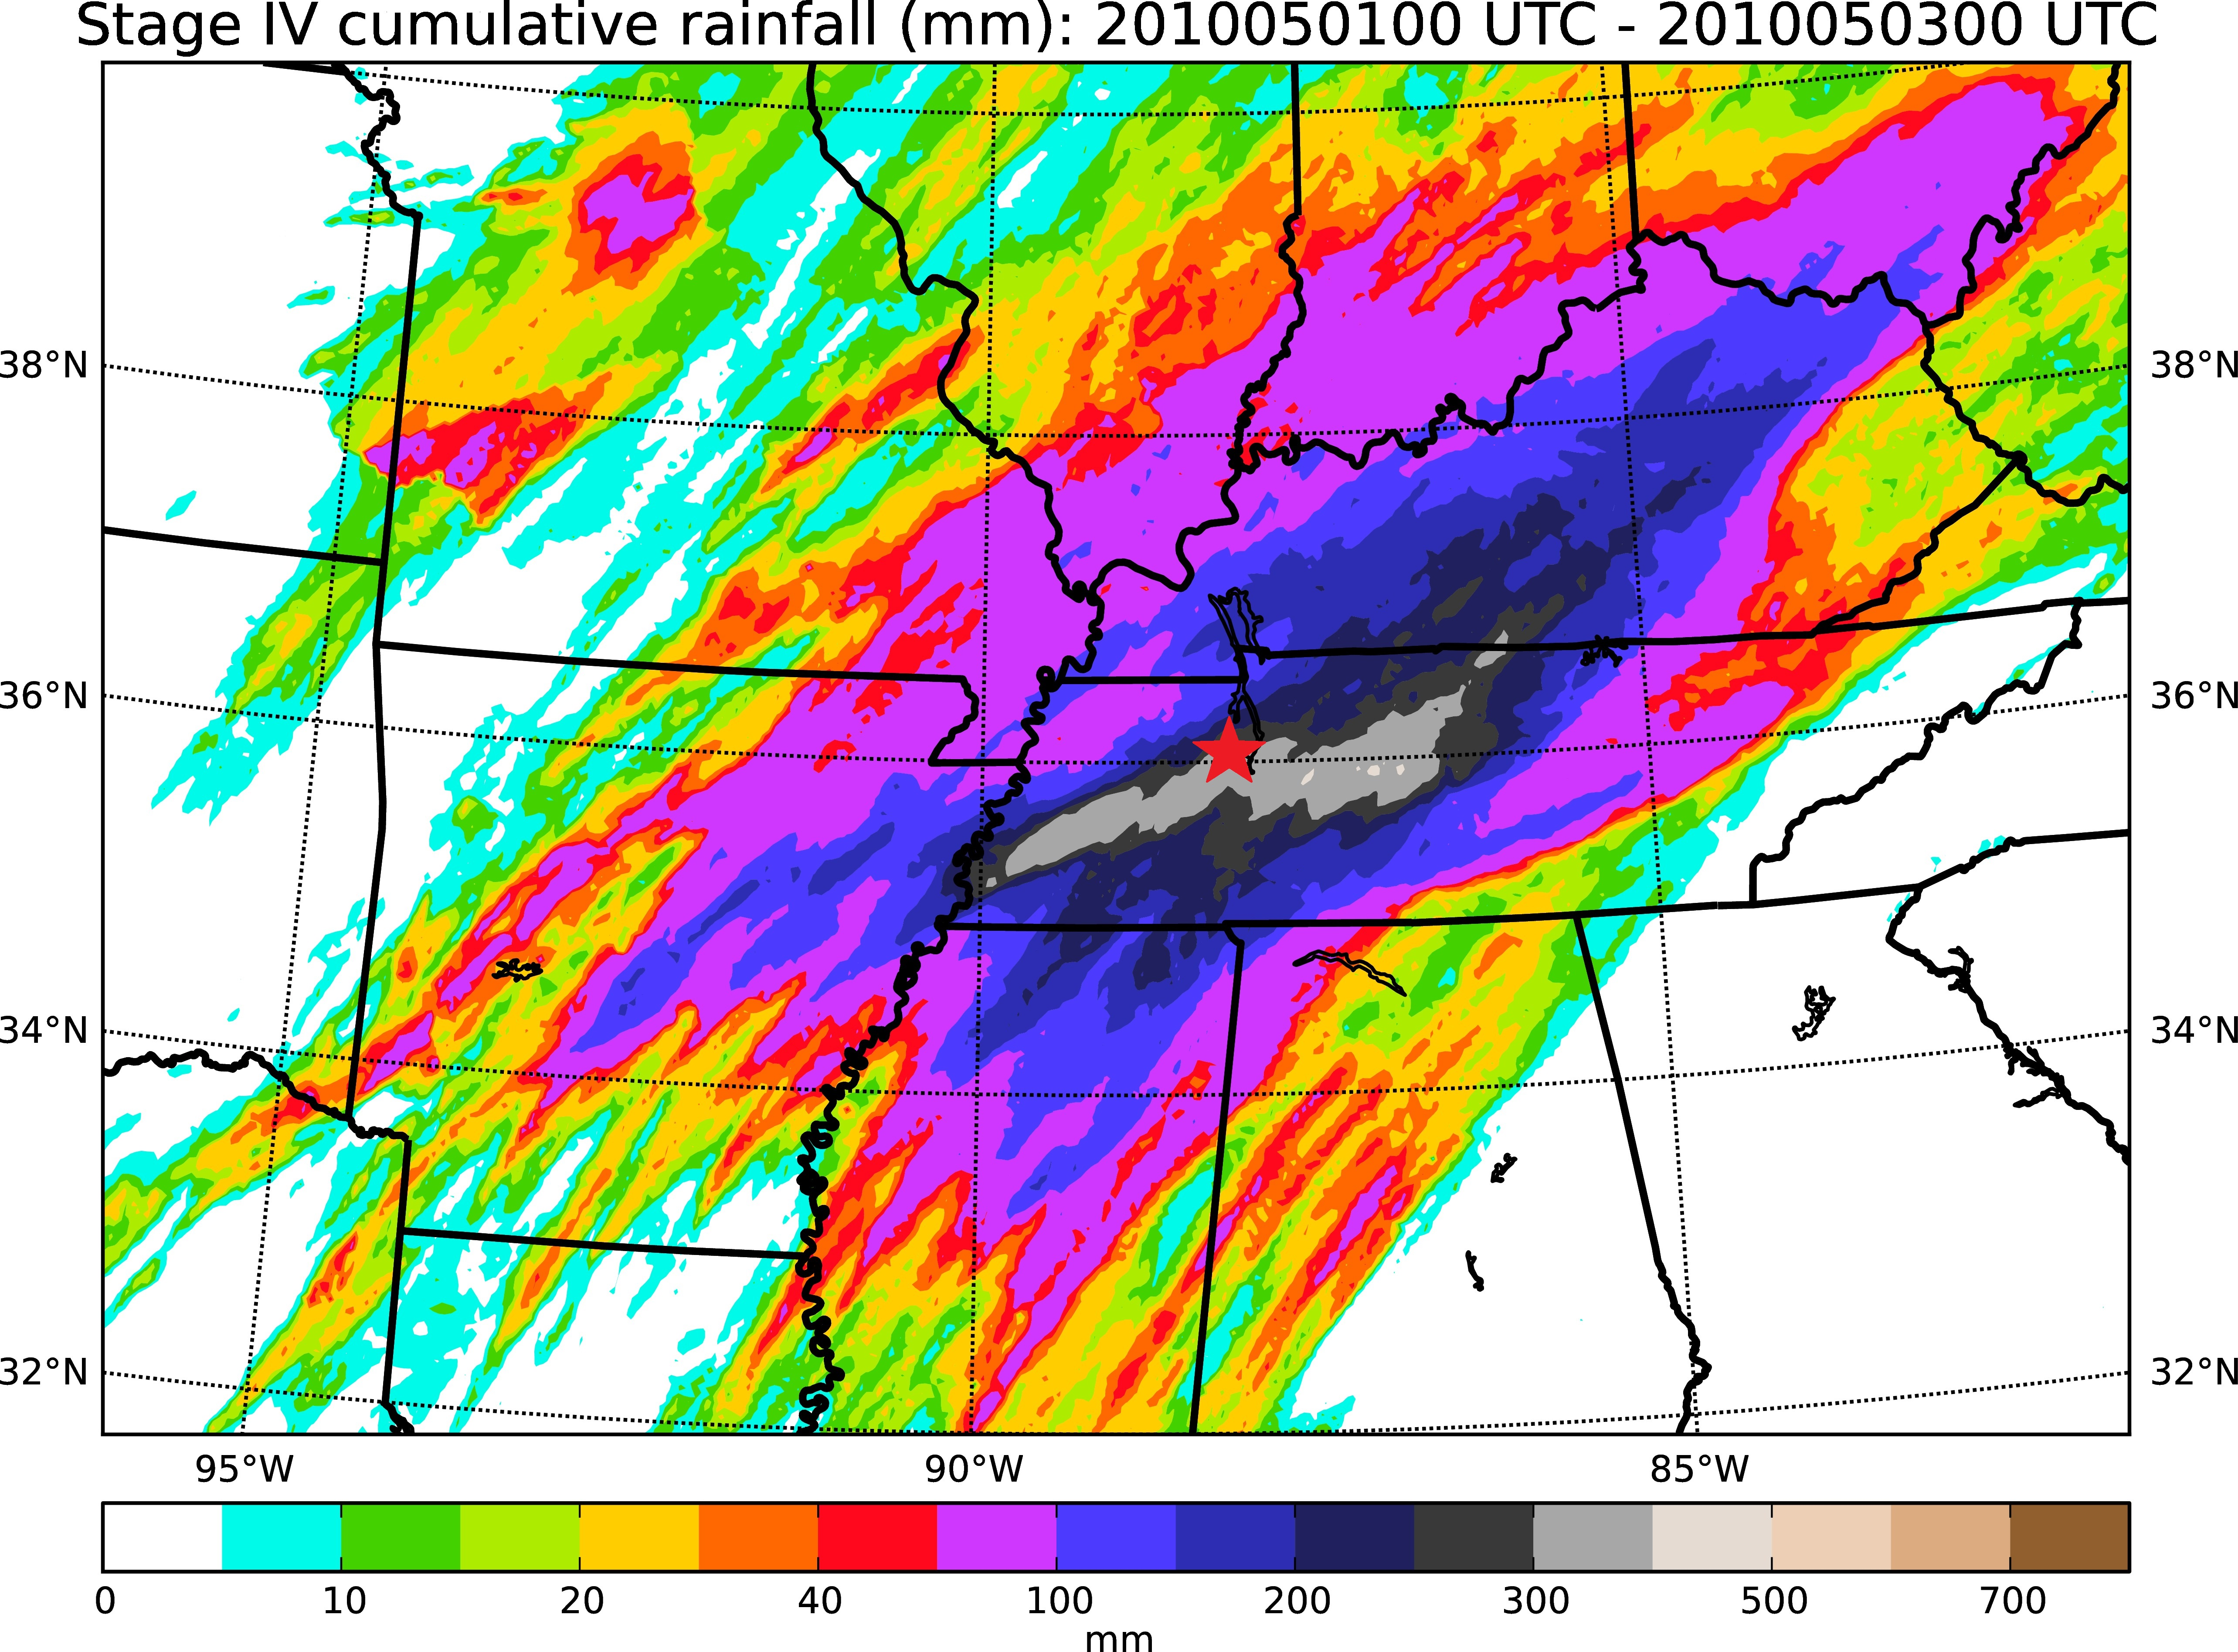
\includegraphics[width=13cm]{pics/ch2/fig1.jpg}
  	\caption{48-hour (0000 UTC 1 May–0000 UTC 3 May, 2010) total rainfall from Stage IV data (unit: mm).}
  	\label{fig:2-1}
\end{figure}

The Nashville 2010 storm was among a series of big storms (tornado 41, 43 and 57) hitting the mid-southern US in the same period. Analysis of reanalysis products suggests that the event was associated with a synoptic system with significant atmospheric moisture. The Atlantic ridging associated with the negative-phase of the North Atlantic Oscillation (NAO) helped amplify and slow the eastward propagating synoptic wave pattern that generated heavy precipitation from mesoscale organized convective systems [\textit{Durkee et al.}, 2012]. An atmospheric river originating from the Intertropical Convergence Zone (ITCZ) in Central America provided the moisture source for this record-breaking event [\textit{Durkee et al.}, 2012]. Surface topography in the Appalachians provided orographic forcing for moisture convergence and land surface heating helped maintain atmospheric instability so precipitation continued until 2 May, 2010. Previous studies have identified several key atmospheric factors such as the superposition of the polar/subtropical jet [\textit{Winters and Martin}, 2014] and the atmospheric river [\textit{Durkee et al.}, 2012; \textit{Moore et al.}, 2012]. Because some elements present in the Nashville 2010 event are common ingredients in other extreme storms, reconstructing this extreme event may serve as an important test case for evaluating the ability of the WRF model for simulating other storms.

\section{The numerical atmospheric model}

WRF model is employed for the big storm reconstruction. WRF is an atmospheric modeling system [\textit{Skamarock et al.}, 2008] that features two non-hydrostatic solvers including the Advanced Research WRF (ARW) core for atmospheric research, and the Non-hydrostatic Mesoscale Model (NMM) core for the operational forecast. In this study we adopted WRF-ARW v3.6.1 for the storm simulation. WRF-ARW has been employed in various big storms studies and demonstrated to be capable of simulating several big storms across the world [\textit{Kumar et al.}, 2008; \textit{Rajeevan et al.}, 2010; \textit{Tan}, 2010; \textit{Chen and Hossain}, 2016].

WRF-ARW is designed for mesoscale meteorological simulation with spatial resolution ranging from 1km to 100km. Accordingly, the time step used in the model varies from seconds to minutes. It simulates the atmospheric motion using compressible, non-hydrostatic Euler equations with consideration of mass, energy and momentum conservation. These equations are formulated and solved using the Arakawa-C grid with terrain-following mass vertical coordinate [\textit{Laprise}, 1992]. WRF-ARW uses various parameterization schemes to estimate the atmospheric processes at sub-grid scale, and atmospheric moisture is considered in various phases in the cloud microphysics parameterization schemes. For example, in the Morrison microphysics scheme, water is considered in vapor, cloud droplets, cloud ice, rain, snow, and graupel/hail phases [\textit{Morrison et al.}, 2009]. This ensures an accurate description of moisture in the air. By default, WRF-ARW model uses USGS or MODIS land use dataset to depict the surface feedback. As a platform, WRF-ARW model provides multiple choices for major physics processes that affect the atmospheric state: cloud microphysics, cumulus process, radiation process, planetary boundary layer process, land surface process. By this modular design, it exhibits great flexibility for mesoscale atmospheric activities across a wide range of temporal and spatial scales, while maintains the capability of incorporating the recent advances in atmospheric sciences.

\section{Experiment design}

Previous studies suggest that the performance of numerical atmospheric models is mostly affected by cloud physics parameterization, model resolution, initial and boundary conditions in the model, as well as the simulation period. Steps below illustrate the workflow needed by engineers to establish the optimal modeling framework based on WRF. A schematic is shown below in Figure \ref{fig:2-2}, and the details of each step are explained below with an example of the Nashville 2010 storm simulation.

\begin{sidewaysfigure}[htbp]
  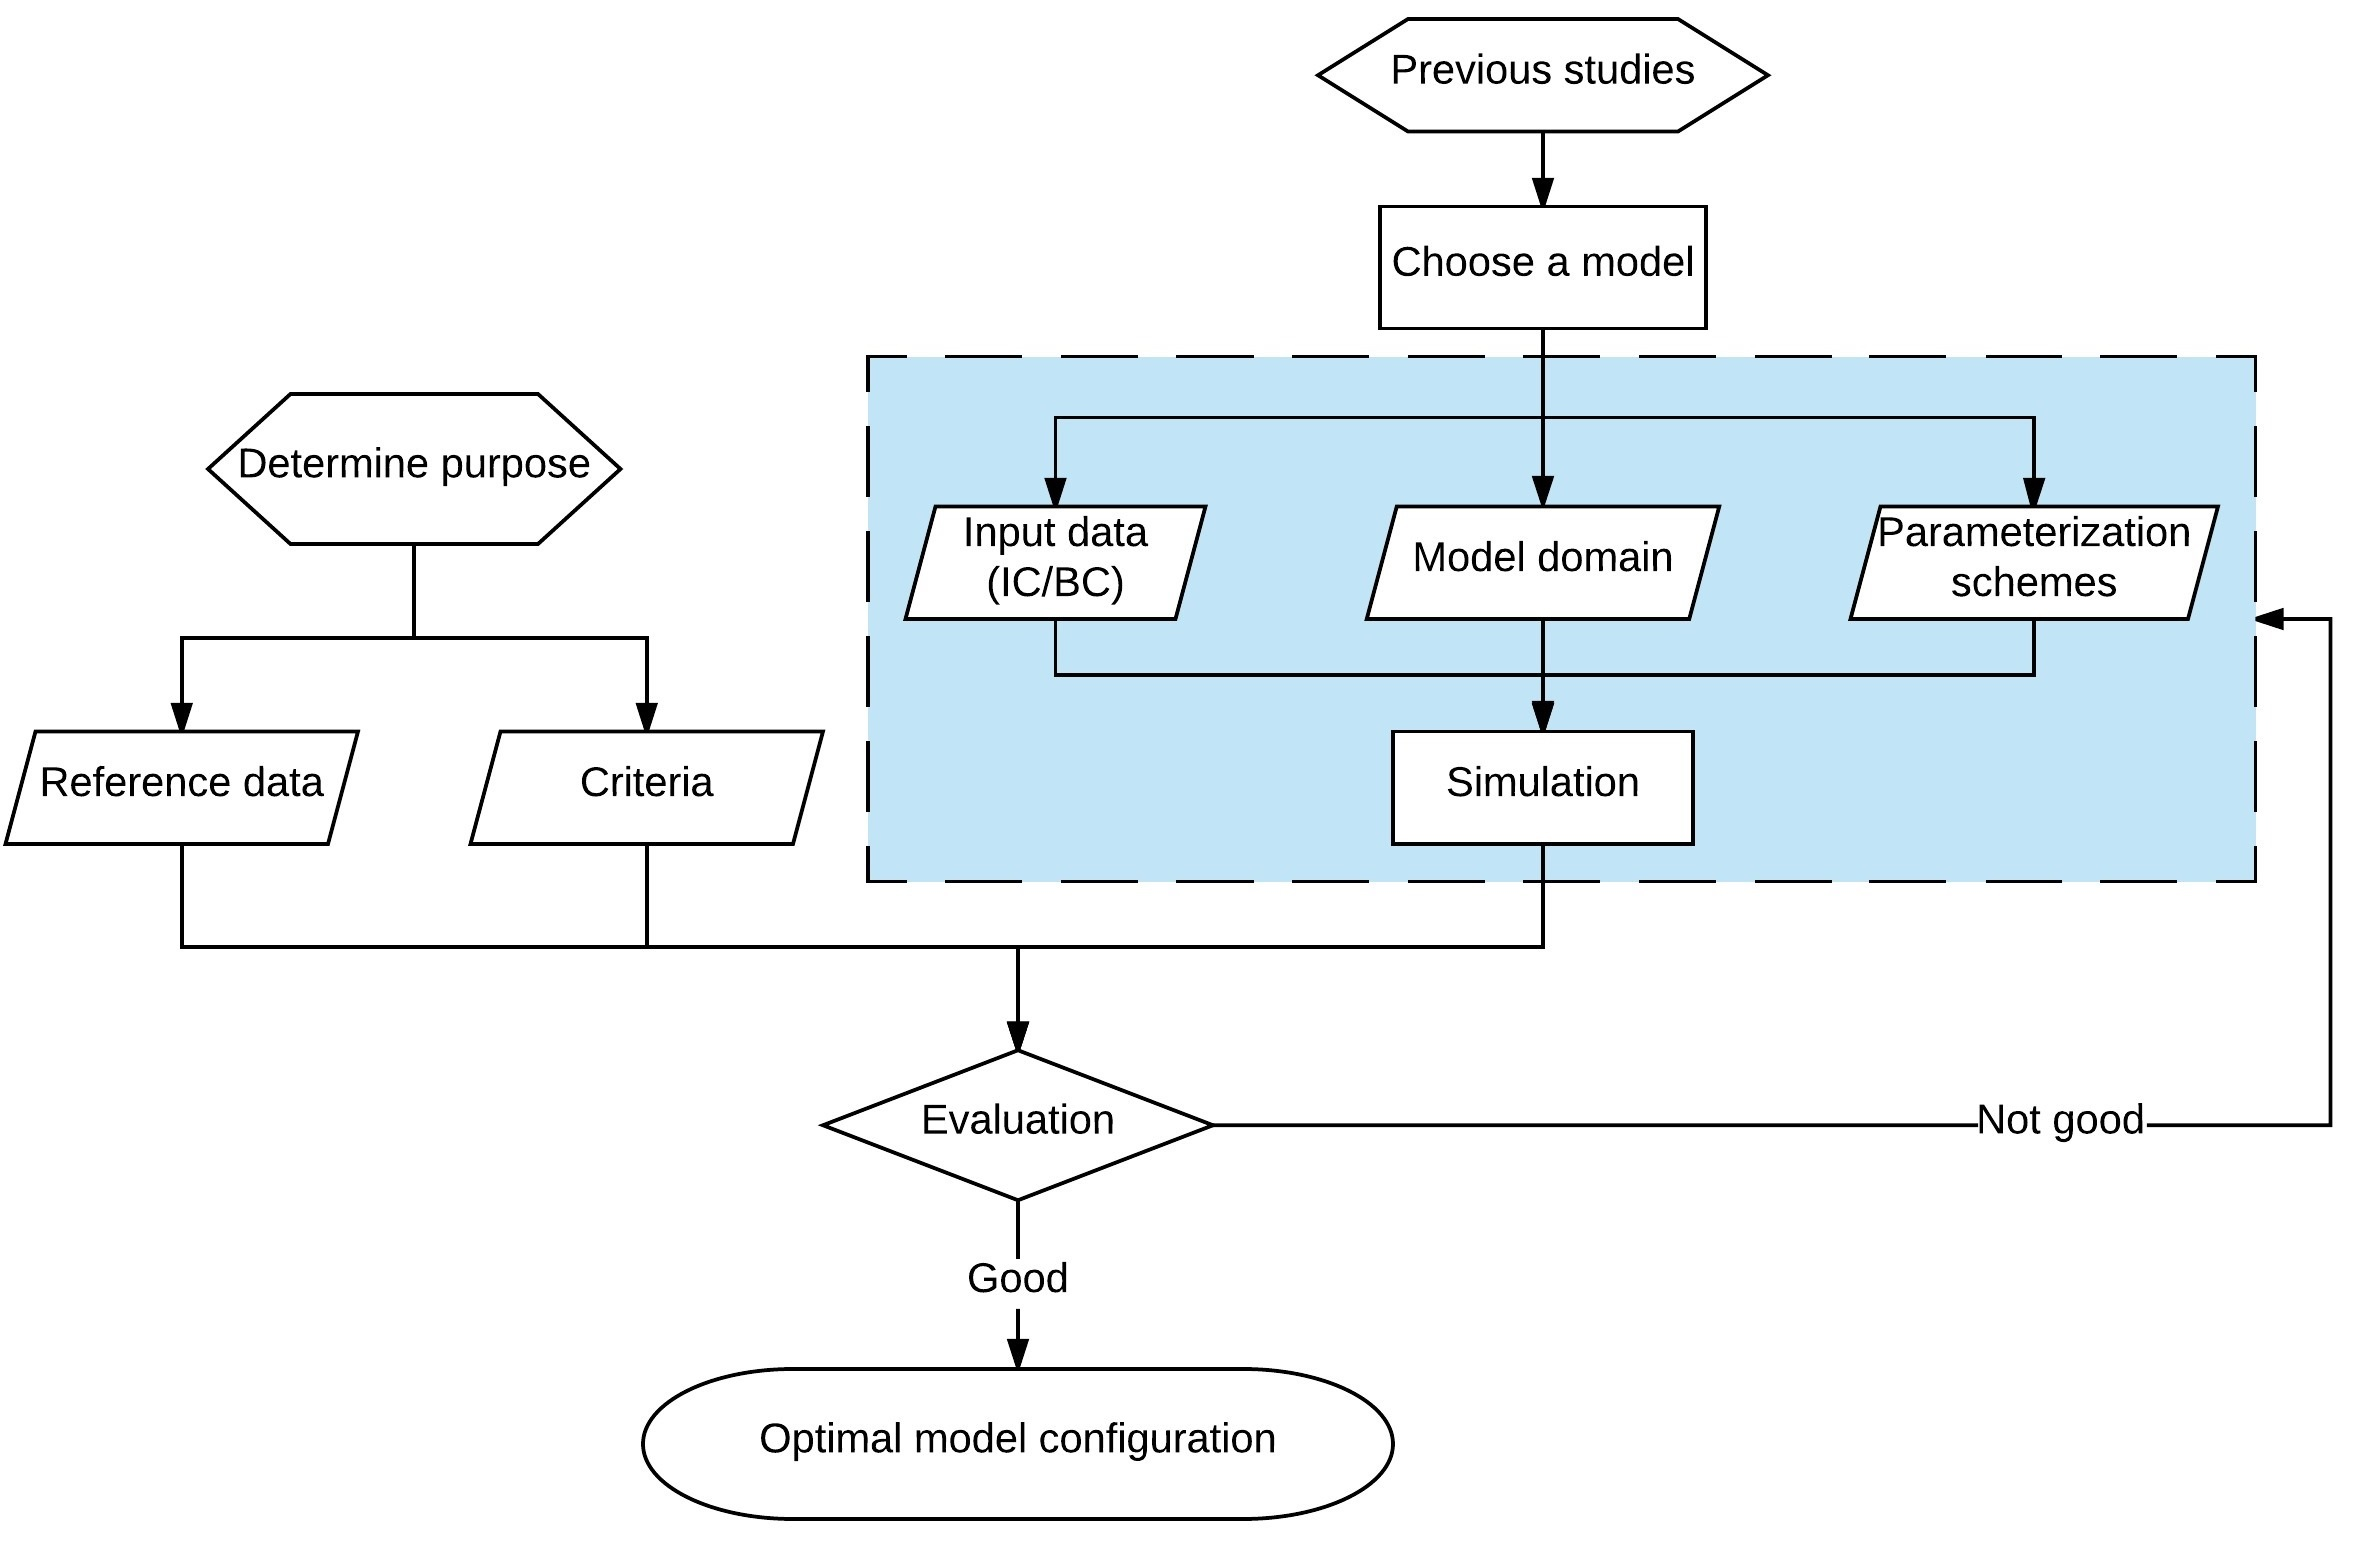
\includegraphics[width=\linewidth]{pics/ch2/fig2.jpg}
  \caption{Generic framework for exploring optimal model configuration for extreme storms}
  \label{fig:2-2}
\end{sidewaysfigure}

1) Study previous modeling efforts to understand the background of the study domain;

2) Determine the atmospheric numerical model(s) of interest;

3) Determine the study domain and simulation period. Prioritize the main physical factors in the model that affect the simulation quality. This can be gained from step 1. Outline the model options (i.e., combination of parameterizations) to be tested;

4) Collect the input data, setup the model and make model runs;

5) Determine the main purpose of the modeling framework and the evaluation criteria. As shown below in the Nashville 2010 case, different purposes of the modeling framework require different criteria, and lead to different configurations in the optimal atmospheric model. Collect the reference data;

6) Evaluate the simulation results using the metric(s) that best serve the purpose.

The Nashville 2010 storm period is May 1-2, 2010, and previous studies [\textit{Mahoney}, 2013] concludes that long spin-up would results in less rainfall during the event. Thus the simulation period is chosen as 0000 UTC 1-3 May 2010. Here we tested 3 configurations of nested domains to test model performance at 15km, 5km, and 1.6km (the latter is referred to as ``2km" for convenience) grid sizes. Figure \ref{fig:2-3} shows the domains in the simulation of the Nashville 2010 storm along with the topography in the domain. The three nested domains in figure \ref{fig:2-3} all centered over western Tennessee. In the first configuration (g15, the 15-km grid D01 domain in the figure), the domain covers the contiguous US at 15km grid spacing. In the second configuration (g5) a D02 domain at 5km resolution is nested inside the larger 15km domain. The third configuration (g2) further includes a D03 domain of 1.6-km spatial resolution to better resolve convection at 1.6km grid spacing. When there is more than one domain involved in the simulation, WRF runs in a two-way nesting mode, which means the coarse grid results are updated using results in finer grids where available. This experiment design allows us to evaluate the impacts of higher resolution achieved through nesting, with the same placement of the outermost lateral boundaries for all simulations. Nominal time steps of 60s, 20s, and 6.7s were used for the 15km, 5km, and 1.6km grids, respectively.  Model outputs are archived hourly between 0000 UTC 1 May 2010 and 0000 UTC 3 May 2010, similar to \textit{Moore et al.} [2012].

\begin{figure}
  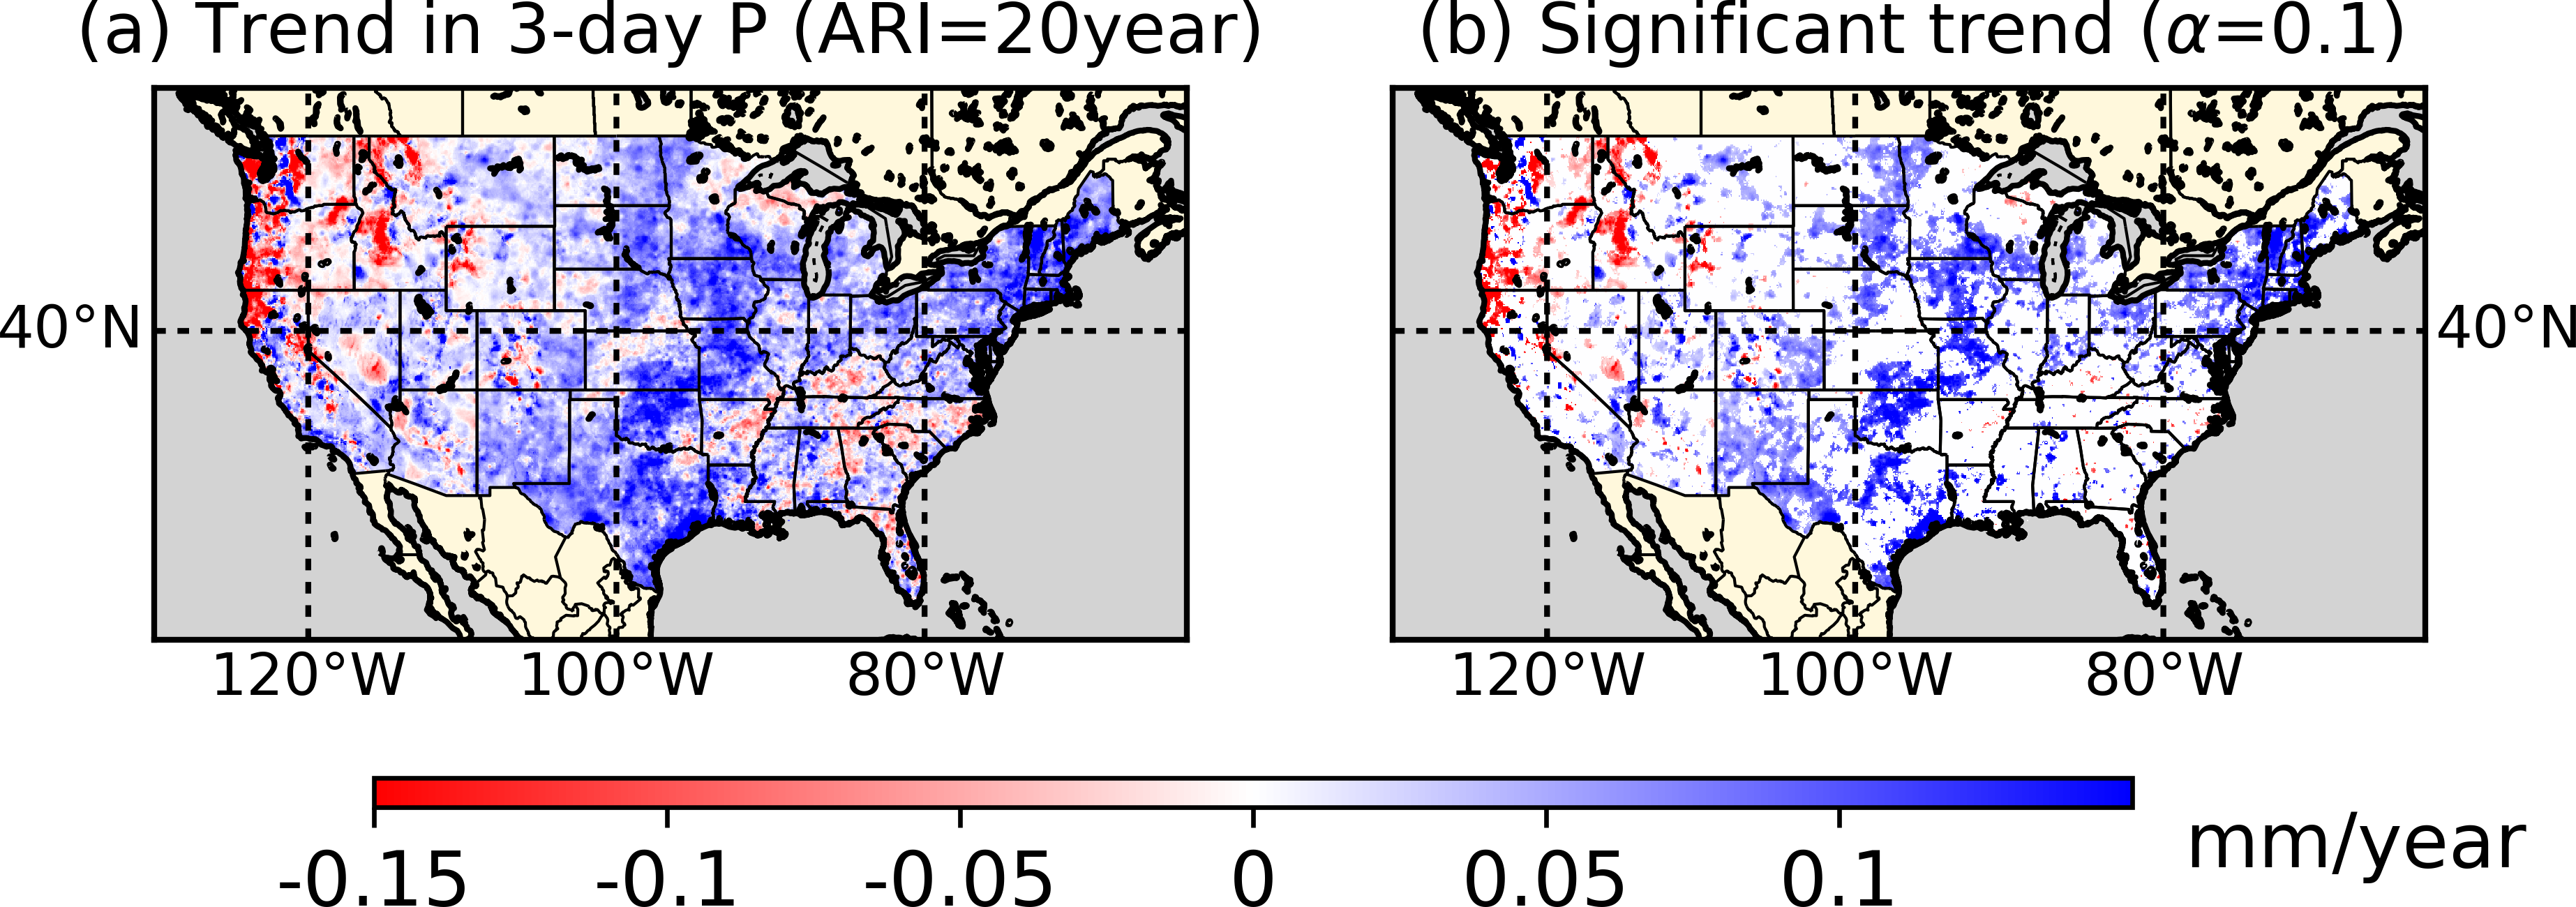
\includegraphics[width=\linewidth]{pics/ch2/fig3.png}
  \caption{Spatial domain in the modeling framework of 2010-Nashville storm.}
  \label{fig:2-3}
\end{figure}

Three sources of data were used to generate IC/BCs: 1) NCEP/DOE reanalysis product (NCEP2) at 2.5-degree resolution; 2) NCEP/NCAR reanalysis product (NNRP) at T62 (209 km) resolution; and 3) North American Mesoscale (NAM) forecast output at T221 (32 km) resolution. For this study the NAM forecast initialized at 0000 UTC 1 May 2010 was used.

Previous studies suggest that precipitation simulation is more sensitive to microphysics and cumulus parameterization schemes than parameterizations for other processes in the model (Del Genio et al. 2005; Pennelly et al. 2014; Zhang and McFarlane 1995). Here we tested three microphysics parameterization schemes for mixed phase clouds including (1) Morrison double moment scheme (coded as ``Morrison" here); (2) New Thompson scheme (``Thompson"); and (3) WSM-5 scheme (``WSM5"). We also evaluated three cumulus parameterization schemes including (1) Kain-Fritsch scheme (coded as ``KF" here); (2) Grell-Devenyi scheme (``GD"); and (3) Grell-Freitas scheme (``GF"). In the nested runs (g5 and g2), cumulus scheme (KF) is used only in the 15km domain, as convection is explicitly resolved at 5km and 2km resolutions. Grell and Freitas (2014) noted that at coarser resolution, the GF scheme functions as a cumulus parameterization to represent the unresolved deep convection, but at a resolution of a few kilometers, deep convection is explicitly resolved and the GF scheme mainly represents shallow convection. Thus another set of simulations are designed to test the scale-aware GF scheme, in which the GF cumulus scheme is applied to all the domains (15km, 5km, 2km) in the nested runs (g5 and g2). Other schemes are fixed in all the experiments, and they are: RRTM longwave radiation scheme; Dudhia shortwave radiation scheme; revised MM5 surface layer scheme; Yonsei University (YSU) planetary boundary layer scheme; Noah land surface scheme.

The total number of combinations of the different options in grid sizes (3), IC/BCs (3), microphysics schemes (3) and cumulus schemes (3 in the g15 runs, 2 in the g5 and g2 runs) amounts to 63 WRF runs designed and conducted for this study.


\section{Evaluation metrics}

An independent precipitation observation data is required for the assessment of the storm simulations. One option is gauge data, since they provide the most accurate estimate of rainfall amount and duration. In some case gauge data may not be available, due to either the age of the storm or the gauges stop working (such as the Nashville international airport station in the Nashville 2010 storm event), the gridded data can be used to validate model results. Here the NEXRAD Stage IV precipitation dataset (Figure \ref{fig:2-1}) is used as the reference in selecting the optimal model configuration, given its high accuracy and good spatial coverage. Cumulative 48-hour rainfall is evaluated by the spatial correlation coefficient between the simulated and Stage IV 48-hour total rainfall. This reveals how the model performs in capturing the rainy area and the spatial heterogeneity of total rainfall. For extreme rainfall events used in engineering analysis, it is important that the numerical model captures the core precipitating areas as accurately as possible. In the validation steps, we used the Livneh daily CONUS near-surface gridded meteorological data [\textit{Livneh et al.}, 2013]. This dataset is developed from gauge observations, and it provides an estimation of daily precipitation. By validating the results using a different reference, we can avoid reference-dependent conclusions.

% table 2.1
\begin{table}[htbp]
	\centering
	\caption{Binary results indices for spatial coverage evaluation metrics}
	%\begin{tabular}{p{2cm}  p{3cm}  p{5cm}   p{5cm}}
	\begin{tabular}{cccc}
		\hline
		\multirow{2}{*}{Simulated} &\multicolumn{3}{c}{Observed}\\
		\cline{2-4}
		&Yes & No & Sum\\
		\hline
		Yes    &  Hits (YY)      &  False alarms YN()       & YY+YN\\
		\hline
		No     &  Misses (NY)    &  Correct Rejection (NN)  & NY+NN\\
		\hline
		Sum    &  YY+NY          &  YN+NN                   & Total=YY+YN+NY+NN\\
		\hline
	\end{tabular}
	\label{table:2-1}
\end{table}


% table 2.2
\begin{table}[htbp]
	\centering
	\caption{Definition of evaluation metrics on storm performance in spatial coverage using metrics from Table \ref{table:2-1}}
	\begin{threeparttable}
		\begin{tabular}{cccc}
			\hline
			Metric  &  Definition   &  Best score   &  Worst score\\
			\hline
			$POD$   &  $\frac{{YY}}{{YY + NY}}$  & 1    & 0\\
			\hline
			$FAR$   &  $\frac{YN}{YY+YN}$        & 0    & 1\\
			\hline
			$Bias$  &  $\frac{YY+YN}{YY+NY}$     & 1    & 0 or $\infty$\\
			\hline
			$HSS$   & $\frac{{2 \times (YY \cdot NN - YN \cdot NY)}}{{(YY + NY)(NY + NN) + (YY + YN)(YN + NN)}}$   &  1    & $-\infty$\\
			\hline
			$TS$    &  $\frac{{YY}}{{YY + NY + YN}}$   &  1    & 0\\
			\hline
			$ETS$   &  $\frac{{YY - Y{Y_{rand}}}}{{YY + NY + YN - Y{Y_{rand}}}}$, where $Y{Y_{rand}} = \frac{{(YY + YN)(YY + NY)}}{{Total}}$   &  1   & -1/3\\
			\hline
		\end{tabular}
		\begin{tablenotes}
			\small
			\item YY (Hits) means both simulation and observation indicate rainfall at the grid/station; YN (False alarm) means only simulation indicates rainfall at the grid/station; NY (Misses) means only observation indicates rainfall at the grid/station; NN (Correct rejection) means neither observation nor simulation indicates rainfall at the grid/station. More details are in Table \ref{table:2-1}. All these metrics are monotonous, except for $Bias$.
		\end{tablenotes}
	\end{threeparttable}
	\label{table:2-2}
\end{table}


Additional metrics we employed include: Probability of Detection ($POD$), False Alert Ratio ($FAR$), frequency Bias ($Bias$), Heidke skill score ($HSS$), Critical Success Index ($CSI$, or $TS$) and Gilbert Skill Score ($GSS$, or $ETS$). They are defined as statistics of the binary result indices in Table \ref{table:2-1}. Table \ref{table:2-2} shows the definitions of these metrics, as well as the ranges of their values. These metrics only measure the accuracy in the coverage of the rainy/non-rainy area. Therefore, when the magnitude of precipitated water matters a lot, it would be better to use the correlation or Root Mean Square Error ($RMSE$) between observed rainfall and simulated rainfall for the period of interest (e.g. 6, 24, 48, and 72 hours in PMP design). This can be done using either station data or gridded data. Other terms worth considering are the storm duration (start time and end time) and peak rainfall (to classify the storm severity). Nash-Sutcliffe model efficiency coefficient ($NS$) is also used to quantify the simulated precipitation. When applied to a ``map", this coefficient can be defined by Eq. (\ref{eq:2-1}), where N is the total number of grid points in the map, $P_o$ is the observed precipitation, $P_m$ is the simulated precipitation. The range of $NS$ is from $-\infty$ to 1, and 1 is the perfect score. Higher NS indicates stronger capacity of the model. These metrics quantitatively evaluate the model performance, thus the recommendations given by these metrics can be applied to engineering practice with confidence [\textit{Bennett et al.}, 2013].

\begin{equation}
	NS = 1 - \frac{{\sum\limits_{n = 1}^N {{{\left( {P_o^n - P_m^n} \right)}^2}} }}{{\sum\limits_{n = 1}^N {{{\left( {P_o^n - \overline {{P_o}} } \right)}^2}} }}
	\label{eq:2-1}
\end{equation}

These metrics measure different aspects of model performance, and provide different recommendations for the ‘best’ combination of parameterizations to support different applications. $POD$ metric as well as storm duration are more useful if the successful forecast of the rainy area is more important, such as the search of possible shelter areas. $FAR$ metric should be weighted more if the cost of emergency relocation is high, in which case we would like to avoid unnecessary effort from areas that are actually not rainy. In the infrastructure design practice, the total amount of rainfall and peak rainfall would be more important. If simulated rainfall data is being used as input to other models (such as hydrological models for streamflow forecasting), then a high spatial correlation or Nash-Sutcliffe coefficient between simulated and observed rainfall would be more desired.
We take into consideration multiple metrics as a ``set" when assessing model performance as no single metric captures all the pertinent performance features. For example, a good numerical model configuration should produce a high probability of detection for rain as well as high critical success index, but a low false alert ratio. We combine several metrics and create a unified score ($US$). The $US$ is defined by Eq. (\ref{eq:2-2}), in which $POD_n$, $FAR_n$ and $CSI_n$ are normalized metrics defined by equation (\ref{eq:2-3}) to (\ref{eq:2-5}). By combining different aspects of model performance into the score, the unified score is used to identify the best combinations for the overall performance reflected by the multi-dimensional metrics that appeal to the engineering infrastructure community [\textit{Sikder and Hossain}, 2016].

\begin{equation}
	US = POD_n^2 - FAR_n^2 + CSI_n^2
	\label{eq:2-2}
\end{equation}

\begin{equation}
	PO{D_n} = \frac{{POD - \min (POD)}}{{\max (POD) - min(POD)}}
	\label{eq:2-3}
\end{equation}

\begin{equation}
	FA{R_n} = \frac{{FAR - \min (FAR)}}{{\max (FAR) - min(FAR)}}
	\label{eq:2-4}
\end{equation}

\begin{equation}
	CS{I_n} = \frac{{CSI - \min (CSI)}}{{\max (CSI) - min(CSI)}}
	\label{eq:2-5}
\end{equation}

\section{Evaluation of reconstruction of the Nashville 2010 extreme storm}

Figure \ref{fig:2-4} shows the observed and simulated 48-hour total rainfall between UTC 0000 1 May 2010 and UTC 0000 3 May 2010. Panel \ref{fig:2-4}(a) is the NEXRAD observation, panel \ref{fig:2-4}(b) is from the WRF simulation using the g5 grids (15km-5km nested grids), NAM IC/BC, Morrison microphysics and KF cumulus parameterization schemes. This is one of the best simulations suggested by the evaluation. Comparison of panel \ref{fig:2-4}(b) with \ref{fig:2-4}(a) indicates that this model setup is able to reconstruct the heavy rainfall area in the mid-west Tennessee. The rainfall amount gradient is properly described by this model setup. Also, the big southwest-northeast pattern of 48-hour total rainfall is clearly captured. Panel \ref{fig:2-4}(c) shows a simulation with moderate scores under evaluation, and \ref{fig:2-4}(d) shows one of the worst simulations. Though all the simulations captured the northeast-southwest oriented rain band, the detailed rainfall distributions from various model configurations differ a lot, thus the evaluation based on the purpose of modeling framework is necessary. The detailed evaluation is shown below as a demo of using different metrics to establish the extreme storm events modeling framework.

\begin{figure}
  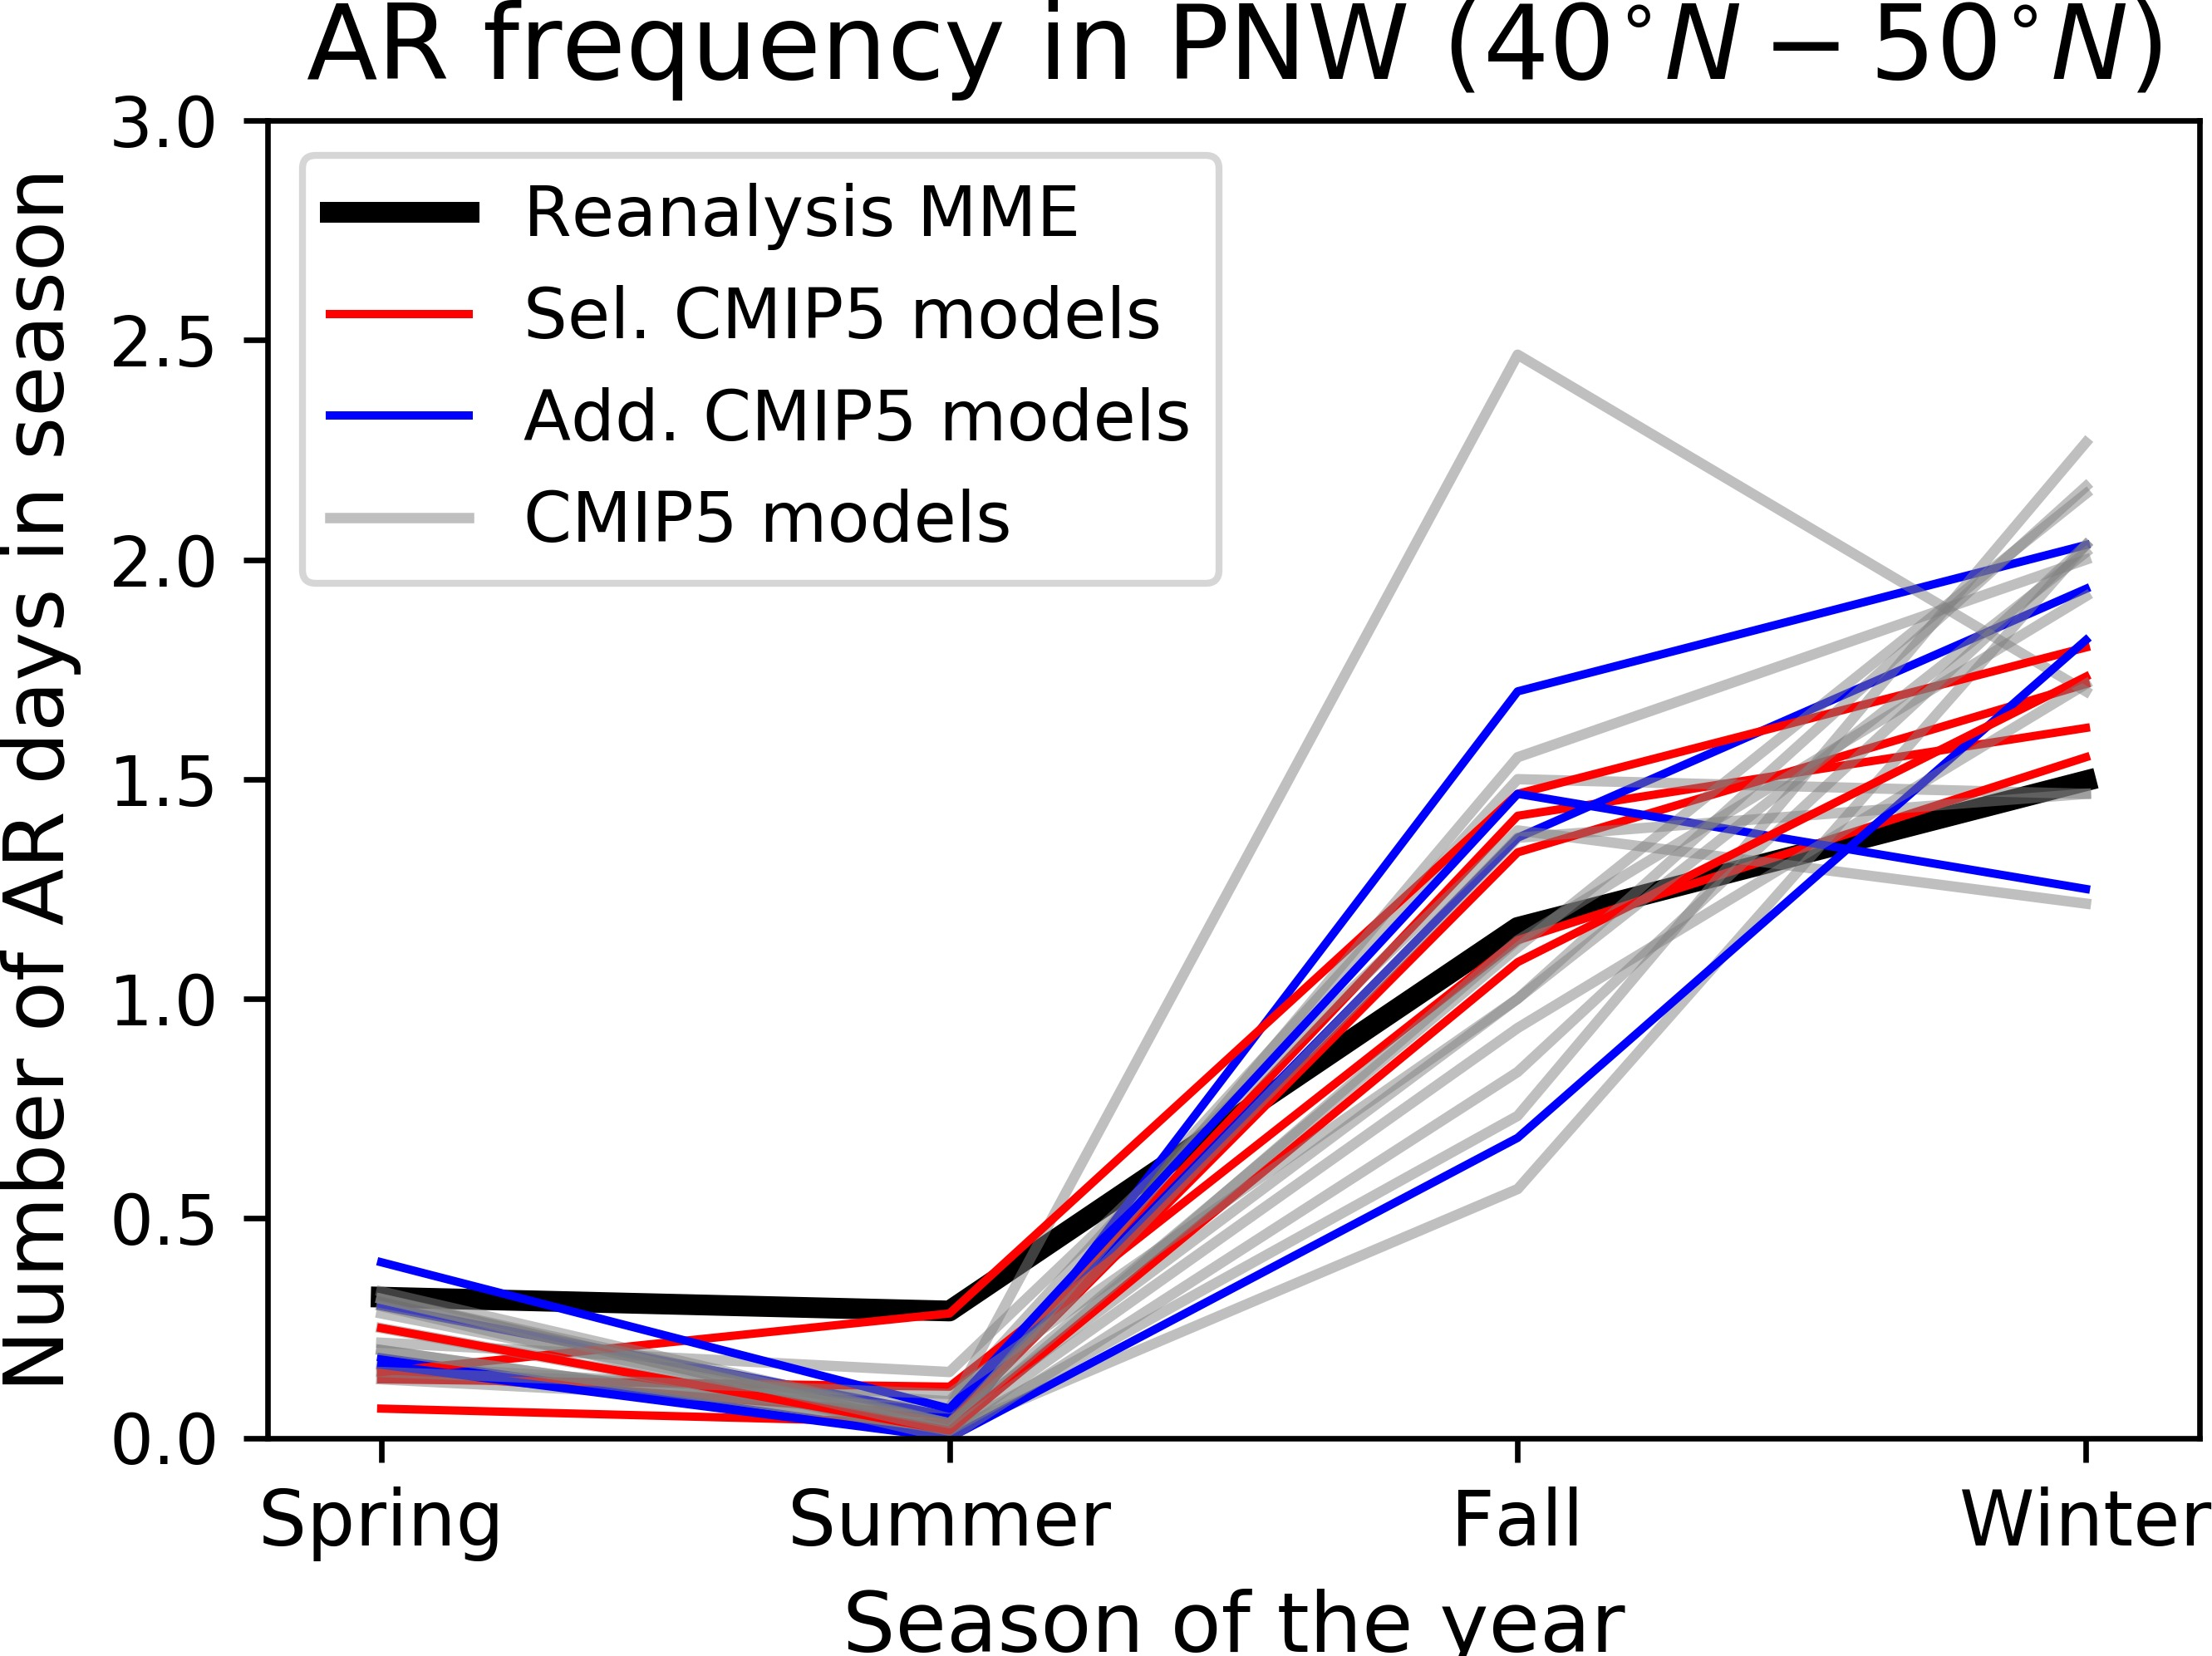
\includegraphics[width=\linewidth]{pics/ch2/fig4.jpg}
  \caption{Stage IV observed and WRF simulated 48-h (0000 UTC 1 May–0000 UTC 3 May, 2010 total rainfall during 2010-Nashville storm event}
  \label{fig:2-4}
\end{figure}

The Stage IV data and simulation results were all conservatively regridded to the 1/16 degree grids within the d03 domain for the following analysis. All the metrics were computed using the results within the box of lat ($31^{\circ}$N, $40^{\circ}$N), lon ($95^{\circ}$W, $84^{\circ}$W), which we will refer to as ``evaluation area".

The total rainfall amount in the event reveals the potential magnitude of the successive flood, and suggests how destructive the storm would be. To evaluate the WRF simulated results, the ratios of simulated total rainfall to the Stage IV total rainfall over the evaluation area were calculated and shown in Table \ref{table:2-3}. Numbers in this table are all normalized using the observed Stage IV 48-hour total rainfall, thus the closer to 1 the more accurately model reconstructs this event. For each grid size, the top three combinations are highlighted in bold in the table.

\begin{table}[htbp]
	\centering
	\caption{Evaluation of averaged 48-hour total rainfall simulated in the evaluation area (normalized using Stage IV observed 48-hour total) in the Nashville 2010 storm event}
	\begin{threeparttable}
		\begin{tabular}{cccccccccc}
			\hline
			\multirow{2}{*}{MP} &\multicolumn{3}{c}{NCEP2} & \multicolumn{3}{c}{NNRP}  & \multicolumn{3}{c}{NAM}\\
			\cline{2-10}
			&KF & GD & GF  & KF & GD & GF & KF & GD & GF\\
			\hline
			% data
			\multicolumn{10}{l}{15-km grids}\\
			%\hline
			Morrison & 0.857 & 0.727 & 0.708 & 0.745 & 0.662 & 0.661 & 0.855 & 0.678 & 0.684\\
			%\hline
			Thompson & \textbf{0.921} & 0.774 & 0.744 & 0.797 & 0.711 & 0.707 & \textbf{0.879} & 0.719 & 0.719\\
			WSM-5    & \textbf{0.866} & 0.754 & 0.740 & 0.753 & 0.705 & 0.698 & 0.855 & 0.712 & 0.718\\
			\hline
			\multicolumn{10}{l}{5-km grids}\\
			Morrison & 0.874 & - & 0.766 & 0.695 & - & 0.680 & 0.890 & - & 0.759\\
			Thompson & 0.856 & - & 0.766 & 0.676 & - & 0.707 & \textbf{0.905} & - & 0.766\\
			WSM-5 & \textbf{0.892} & - & 0.787 & 0.707 & - & 0.706 & \textbf{0.899} & - & 0.793\\
			\hline
			\multicolumn{10}{l}{2-km grids}\\
			Morrision & 0.827 & - & 0.780 & 0.692 & - & 0.663 & \textbf{0.882} & - & 0.816\\
			Thompson & 0.773 & - & 0.723 & 0.636 & - & 0.603 & 0.855 & - & 0.781\\
			WSM-5 & \textbf{0.841} & - & 0.794 & 0.683 & - & 0.648 & \textbf{0.898} & - & 0.829\\
			\hline
			
		\end{tabular}	
		\begin{tablenotes}
			\small
			\item  Bold numbers are the top 3 scores with the best performance within each grid resolution.
		\end{tablenotes}
	\end{threeparttable}
	\label{table:2-3}
\end{table}

All of these combinations tend to underestimate the total rainfall in the evaluation area. However, the best results (such as g15-NCEP2-Thompson-KF and g5-NAM-Thompson-KF) are pretty close to the observed amount, with the difference within 10\%. Also, the performance of NCEP2 performance is comparable to those of NAM IC/BC, both of which are significantly better than NNRP IC/BC. The simulated total rainfall amount is sensitive to cumulus scheme, as the difference in KF results from NCEP2 and NAM IC/BC is less than 7\%, while difference due to cumulus schemes are larger than 10\%. It is also worth noting that the best results come from coarser resolution. Thus for total rainfall estimation, the optimal framework would go up to only 5km resolution.

Table \ref{table:2-4} shows the spatial correlations and RMSEs between the simulated 48-hour total rainfall maps and the Stage IV total rainfall map. Values in parentheses are the RMSE results. For each grid size, the top three combinations in correlation coefficient are highlighted in bold in the table. Similarly, the top three combinations in RMSE are also bolded in the table, and they are exactly those deriving the best spatial correlation. At all 3 grid scales, NAM provides the best estimates of the 48-hour total rainfall. Within each IC/BC category, the difference from different microphysics schemes is not huge (usually only within 20\% of the score), but different cumulus parameterization schemes have significant impacts on the precipitation simulation quality. This is especially notable in the simulations driven by the NCEP2 IC/BC where the spatial correlation ranges from ~0.2 (GF scheme) to ~0.6 (KF scheme), and the correlations with the KF scheme are always higher than those with the GF scheme. We also note that the g5-NAM-Morrison-KF case (panel \ref{fig:2-4}b) produced the best spatial correlation among all the tested cases. Based on table 3, NAM IC/BC and KF cumulus scheme is recommended for storm reconstructions that address the spatial distribution of the cumulative rainfall (such as PMP design). However, since this result is based only on the cumulative rainfall, it does not reveal temporal evolution information.

\begin{table}[htbp]
	\centering
	\caption{Spatial correlation and RMSE between simulated and Stage IV reference 48-hour cumulative rainfall distribution in the Nashville 2010 storm event}
	\begin{threeparttable}
		\begin{tabular}{cccccccccc}
		\hline
		\multirow{2}{*}{MP} & \multicolumn{3}{c}{NCEP2} & \multicolumn{3}{c}{NNRP} & \multicolumn{3}{c}{NAM}\\
		\cline{2-10}
		& KF & GD & GF & KF & GD & GF & KF & GD & GF\\
		\hline
		\multicolumn{10}{l}{15-km grids}\\
		Morrisoin & 0.364 &0.344 &0.231 &0.259 &0.345 &0.139 & \textbf{0.597} &0.488 &0.471\\
		&(65.0) &(66.4) &(69.4) &(69.4) &(66.8)  &(71.6) &\textbf{(55.4)} &(62.2) &(62.7)\\
		Thompson & 0.359 &0.368 &0.254 &0.249 &0.344 &0.125 &\textbf{0.606} &0.516 &0.516\\
		&(65.5) &(65.2) &(68.4) &(69.8) &(66.2) &(71.6) &\textbf{(54.7)} &(60.5) &(60.5)\\
		WSM-5 &  0.365 & 0.362 & 0.271 & 0.261 & 0.361 & 0.122 & \textbf{0.589} & 0.485 & 0.418\\
		& (64.9) & (65.6) & (68.1) & (69.4) & (65.8) & (71.8) & \textbf{(55.8)} & (61.8) & (64.2)\\
		\hline
		\multicolumn{10}{l}{5-km grids}\\
		Morrison & 0.455 & - & 0.171 & 0.311 & - & 0.154 & \textbf{0.773} & - & 0.500\\
		& (62.1) && (71.3) & (69.1) && (71.1) & \textbf{(43.8)} && (60.6)\\
		Thompson & 0.335 & - & 0.216 & 0.334 & - & 0.159 & \textbf{0.698} & - & 0.509\\
		& (68.1) && (69.4) & (68.5) && (70.7) & \textbf{(49.2)} && (60.2)\\
		WSM-5 & 0.322 & - & 0.220 & 0.337 & - & 0.172 & \textbf{0.700} & - & 0.537\\
		& (68.9) && (70.0) & (68.0) && (70.3) & \textbf{(49.2)} && (58.7)\\
		\hline
		\multicolumn{10}{l}{2-km grids}\\
		Morrison & 0.596 & - & 0.527 & 0.289 & - & 0.293 & \textbf{0.766} & - & \textbf{0.705}\\
		& (55.6) & & (59.3) & (70.1) & & (70.2) & \textbf{(44.4)} & & \textbf{(49.4)}\\
		Thompson & 0.490 & - & 0.380 & 0.277 & - & 0.302 & 0.697 & - & 0.644\\
		& (61.0) & & (65.8) & (70.1) & & (69.3) & (49.6) & & (53.6)\\
		WSM-5 & 0.482 & - & 0.435 & 0.318 & - & 0.313 & \textbf{0.708} & - & 0.623\\
		& (61.4) & & (63.8) & (68.4) & & (68.7) & \textbf{(48.8)} & & (54.6)\\
		\hline
		\end{tabular}
		\begin{tablenotes}
			\small
			\item Values in parentheses are $RMSE$ (unit: mm/day). Bold numbers are the top 3 scores with the best performance (highest correlation or lowest RMSE) within each grid resolution.
		\end{tablenotes}
	\end{threeparttable}
	\label{table:2-4}
\end{table}

At 5km and 2km grid scale, all the combinations produce stronger correlations. As we can see in the following analysis, NAM often produces the best quantitative evaluation values in the finer grids. The top combinations for the 5km grids and 2km grids are similar. The difference among the best correlation results at the 3 different grid scales is not significant. In general, higher resolution simulations are able to capture finer scale features, although the improvement from 5km to 2km is marginal.

In certain types of engineering infrastructure analyses, it is important to know both the location and period of the storm event. A better picture of the spatial-temporal structure of the storm would help make better operation plans for the drainage systems, for example. To better evaluate the simulated spatial-temporal structures of the storm, quantitative scores were computed for the 63 simulations. Unlike the calculation of spatial correlation using rainfall total, the computation here used hourly rainfall data. Figure \ref{fig:2-5} visualizes the evaluation on the spatial coverage of hourly rainfall simulated by WRF. Blank in the panels means the corresponding combination was not tested (similar to the ``-" in Table \ref{table:2-3}). Panel \ref{fig:2-5}(a) shows the $POD$, with greater values representing more skillful simulations. Similarly, panel \ref{fig:2-5}(b) shows the $FAR$ (lower values are better). $POD$ reflects the probability of rainfall grid points being successfully simulated as ``rainy" by the numerical model. FAR evaluates the simulation accuracy of non-rainy regions, so combining it with POD can provide a better assessment of the simulation quality.

\begin{figure}[htbp]
  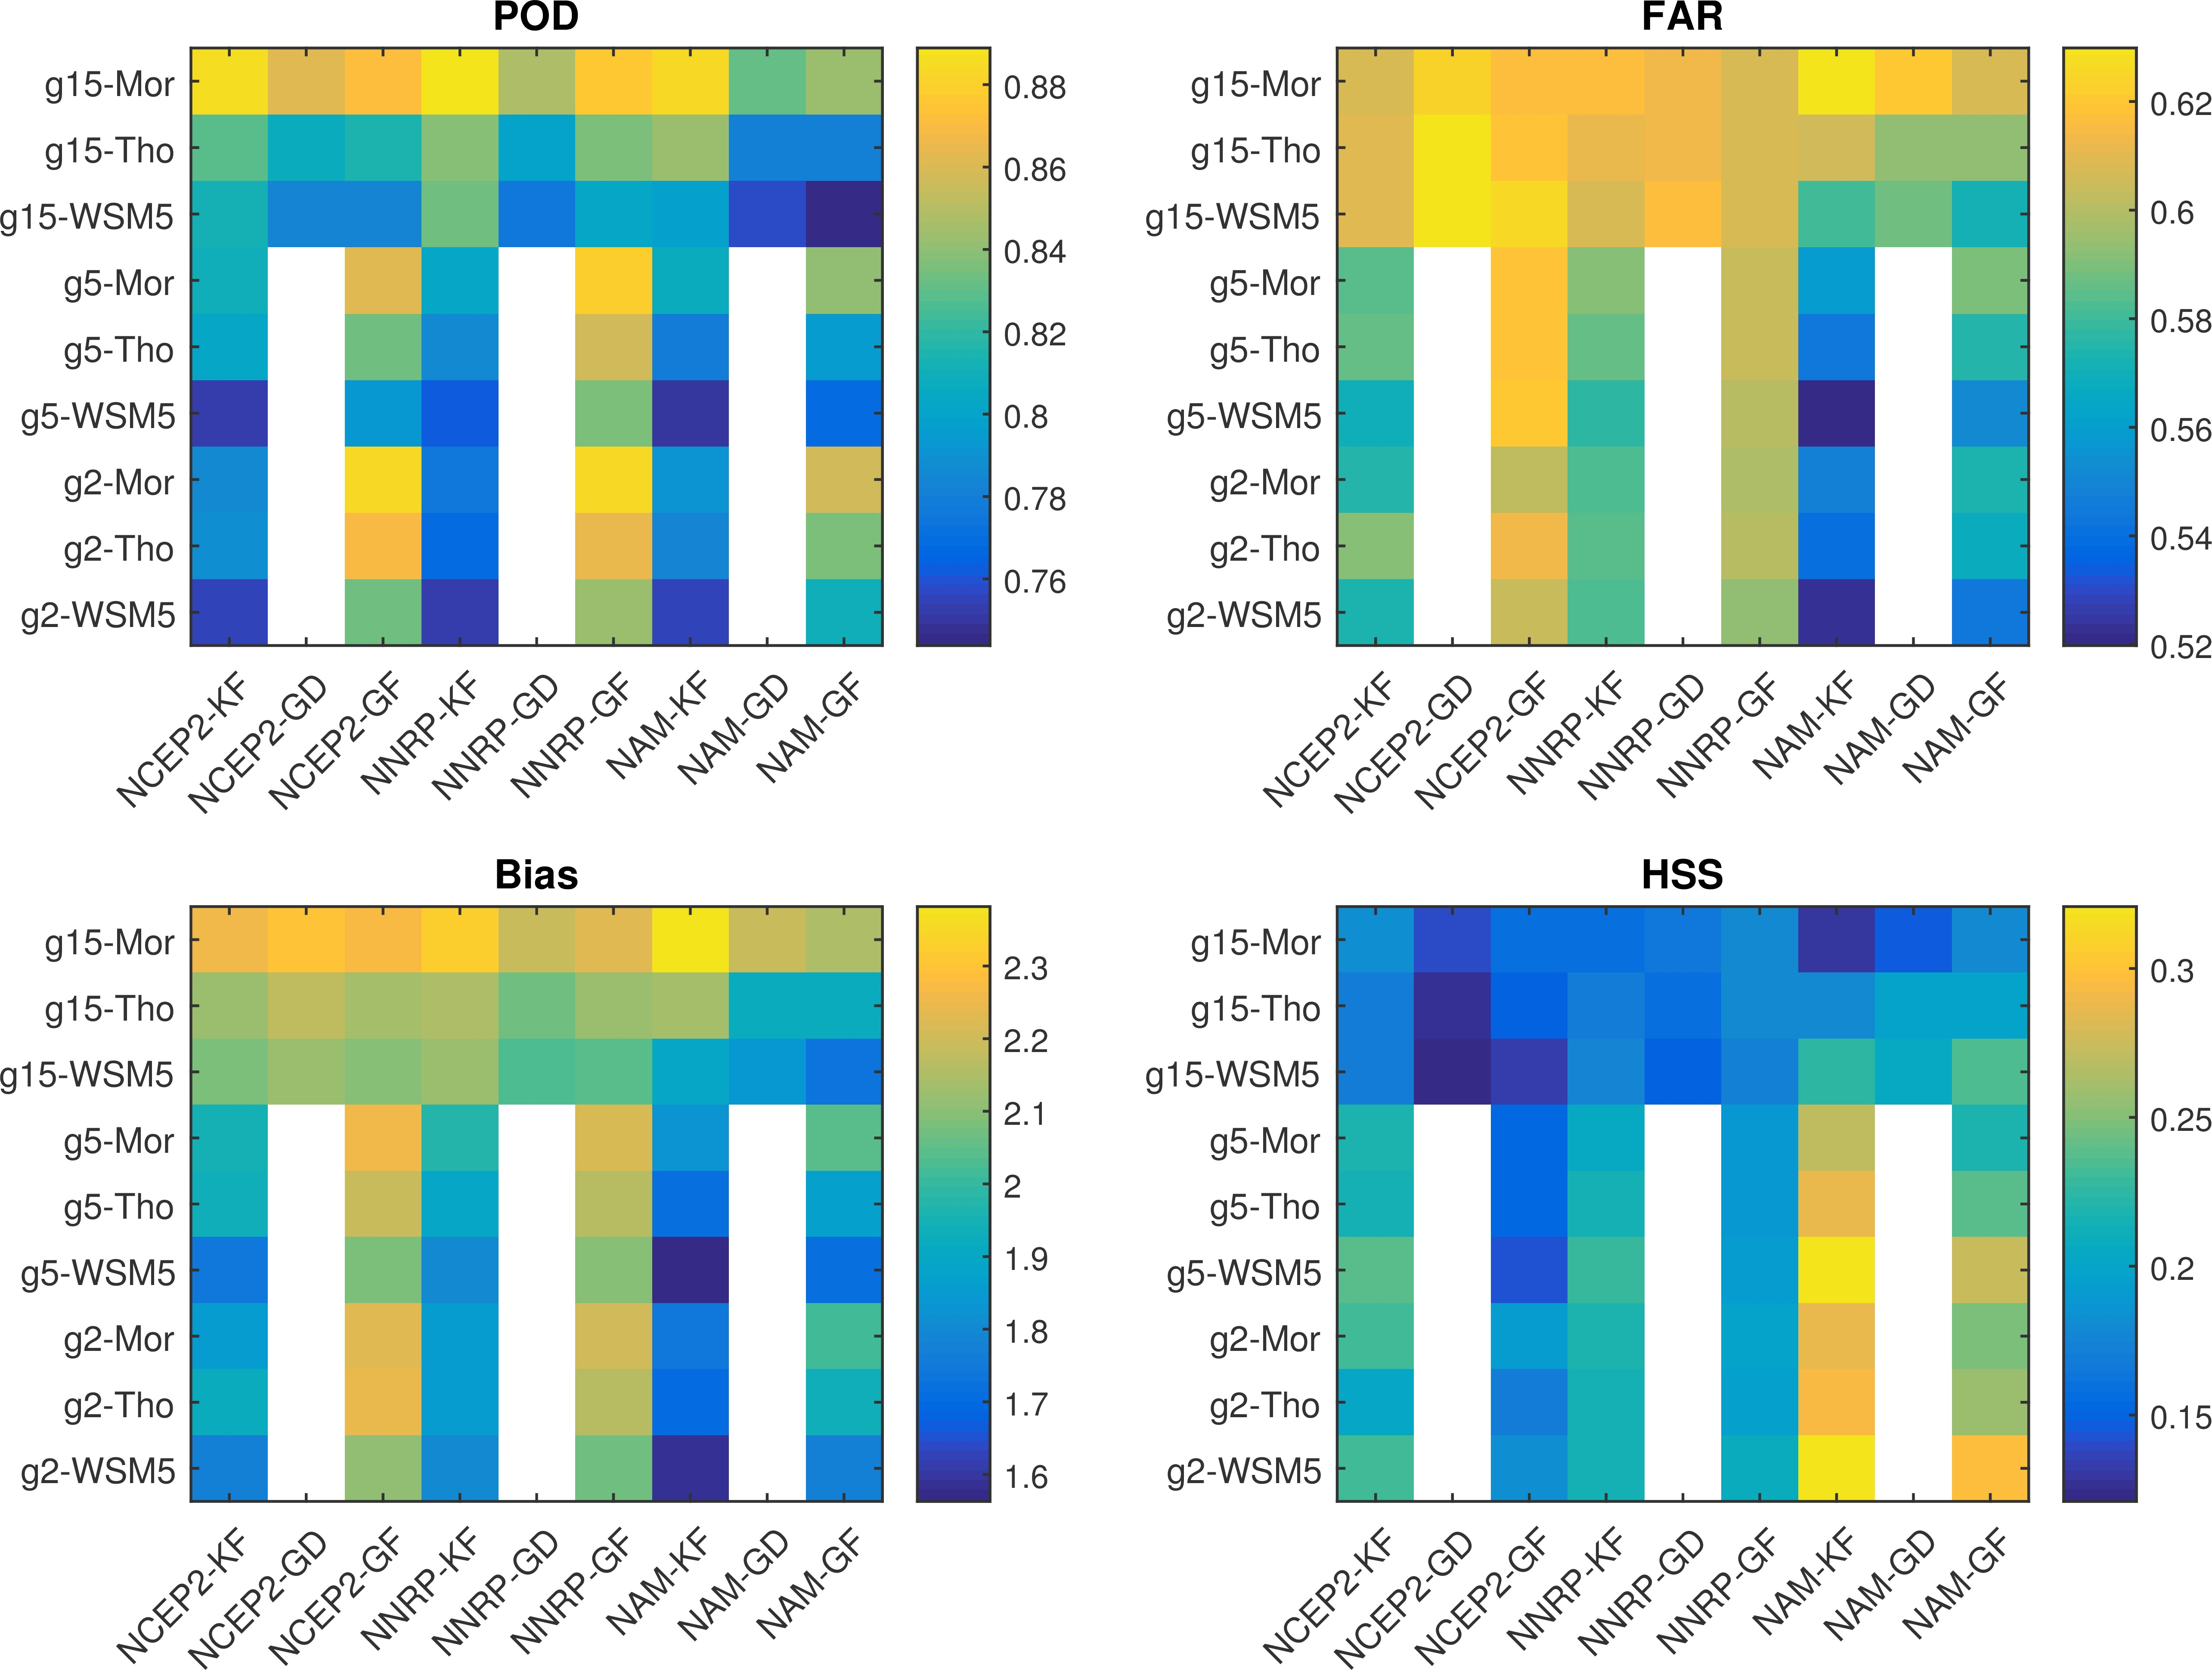
\includegraphics[width=\linewidth]{pics/ch2/fig5.jpg}
  \caption{Evaluation of spatial coverage simulated by WRF. Panel (a) shows $POD$, (b) shows $FAR$, (c) shows $Bias$, (d) shows $HSS$ scores.}
  \label{fig:2-5}
\end{figure}

The general information from panels \ref{fig:2-5}(a) and \ref{fig:2-5}(b) suggests that as the numerical model takes advantage of the finer grids, the simulation quality usually improves. The g15 grid shows somewhat better $POD$ than some of the g5 and g2 results, which is possible because POD only measures how complete the observed rainfall area is covered by the simulation. Panel \ref{fig:2-5}(a) suggests that the Morrison microphysics scheme tends to overestimate rainfall coverage, and this is supported by the higher $FAR$ values in panel \ref{fig:2-5}(b). Compared with the g15 grid, finer grids simulations are able to reduce the likelihood of false alert: The range of the best three $FAR$ scores in the g15 grid is [0.571, 0.588], which is less skillful than the g5 results of [0.520, 0.551]. Similar to the findings from the spatial correlation and total rainfall analyses, the biggest difference in the $FAR$ comes from the choice of IC/BCs: NAM outperforms others at both coarser and finer grids. Also, the WSM-5 scheme tends to produce less spatial extent of rainfall, so it performs better for the $FAR$ score.

Panel \ref{fig:2-5}(c) shows the frequency bias scores. A bias score larger than 1 means the model overestimates the rainfall coverage, and a score less than 1 suggests an underestimation. As WRF is applied in the finer grids, the bias scores steadily converge to 1. All microphysics schemes benefit from the use of the finer grids. All of the bias scores are larger than 1, which indicates that all the models overestimate the rainfall area. Since the total rainfall amount analysis suggests that all the models underestimate the total rainfall amount, the simulated picture is most likely to be expanded rainy area with rain rate smaller than the observed rate. This is confirmed by comparing panel \ref{fig:2-4}(b) to \ref{fig:2-4}(a). Panel \ref{fig:2-5}(d) presents the $HSS$, with higher scores indicating better simulations. For a simulation with non-zero capability in forecasting/simulation, the $HSS$ must be greater than 0. Panel \ref{fig:2-5}(d) shows that all the 63 simulations have some capabilities for forecasting/simulation. Similar to the $FAR$ scores, NAM IC/BC performs best at both coarser and finer grids. The improvement from the g15 to g5 grids is significant (about 20\% increase), but the even finer g2 grid does not provide further improvement. Thus the 5km grid is an acceptable compromise for PMP simulation as it does not compromise simulation quality at the expense of reduced computational burden. In terms of microphysics schemes, WSM-5 is best for both the finer and coarse grids. In the coarse grid, KF cumulus scheme is also a good choice when combined with the Morrison or new Thompson cumulus schemes.

Figure \ref{fig:2-6} shows the evaluation based on metrics that considers multiple aspects of the rainfall simulation quality. Panel \ref{fig:2-6}(a) shows the $CSI$ grades (the higher the better). Any skillful forecast/simulation should have greater than 0 grades. Panel \ref{fig:2-6}(c) shows the $GSS$ grades (the higher the better). $GSS$ improves $CSI$ grades by taking into account the randomness of the observation, and it also requires a positive grade for the simulation to be considered skillful. The largest differences come from the choice of the IC/BC data source, and it is obvious that WSM-5 is the winning microphysics scheme at various grids.

\begin{figure}[htbp]
  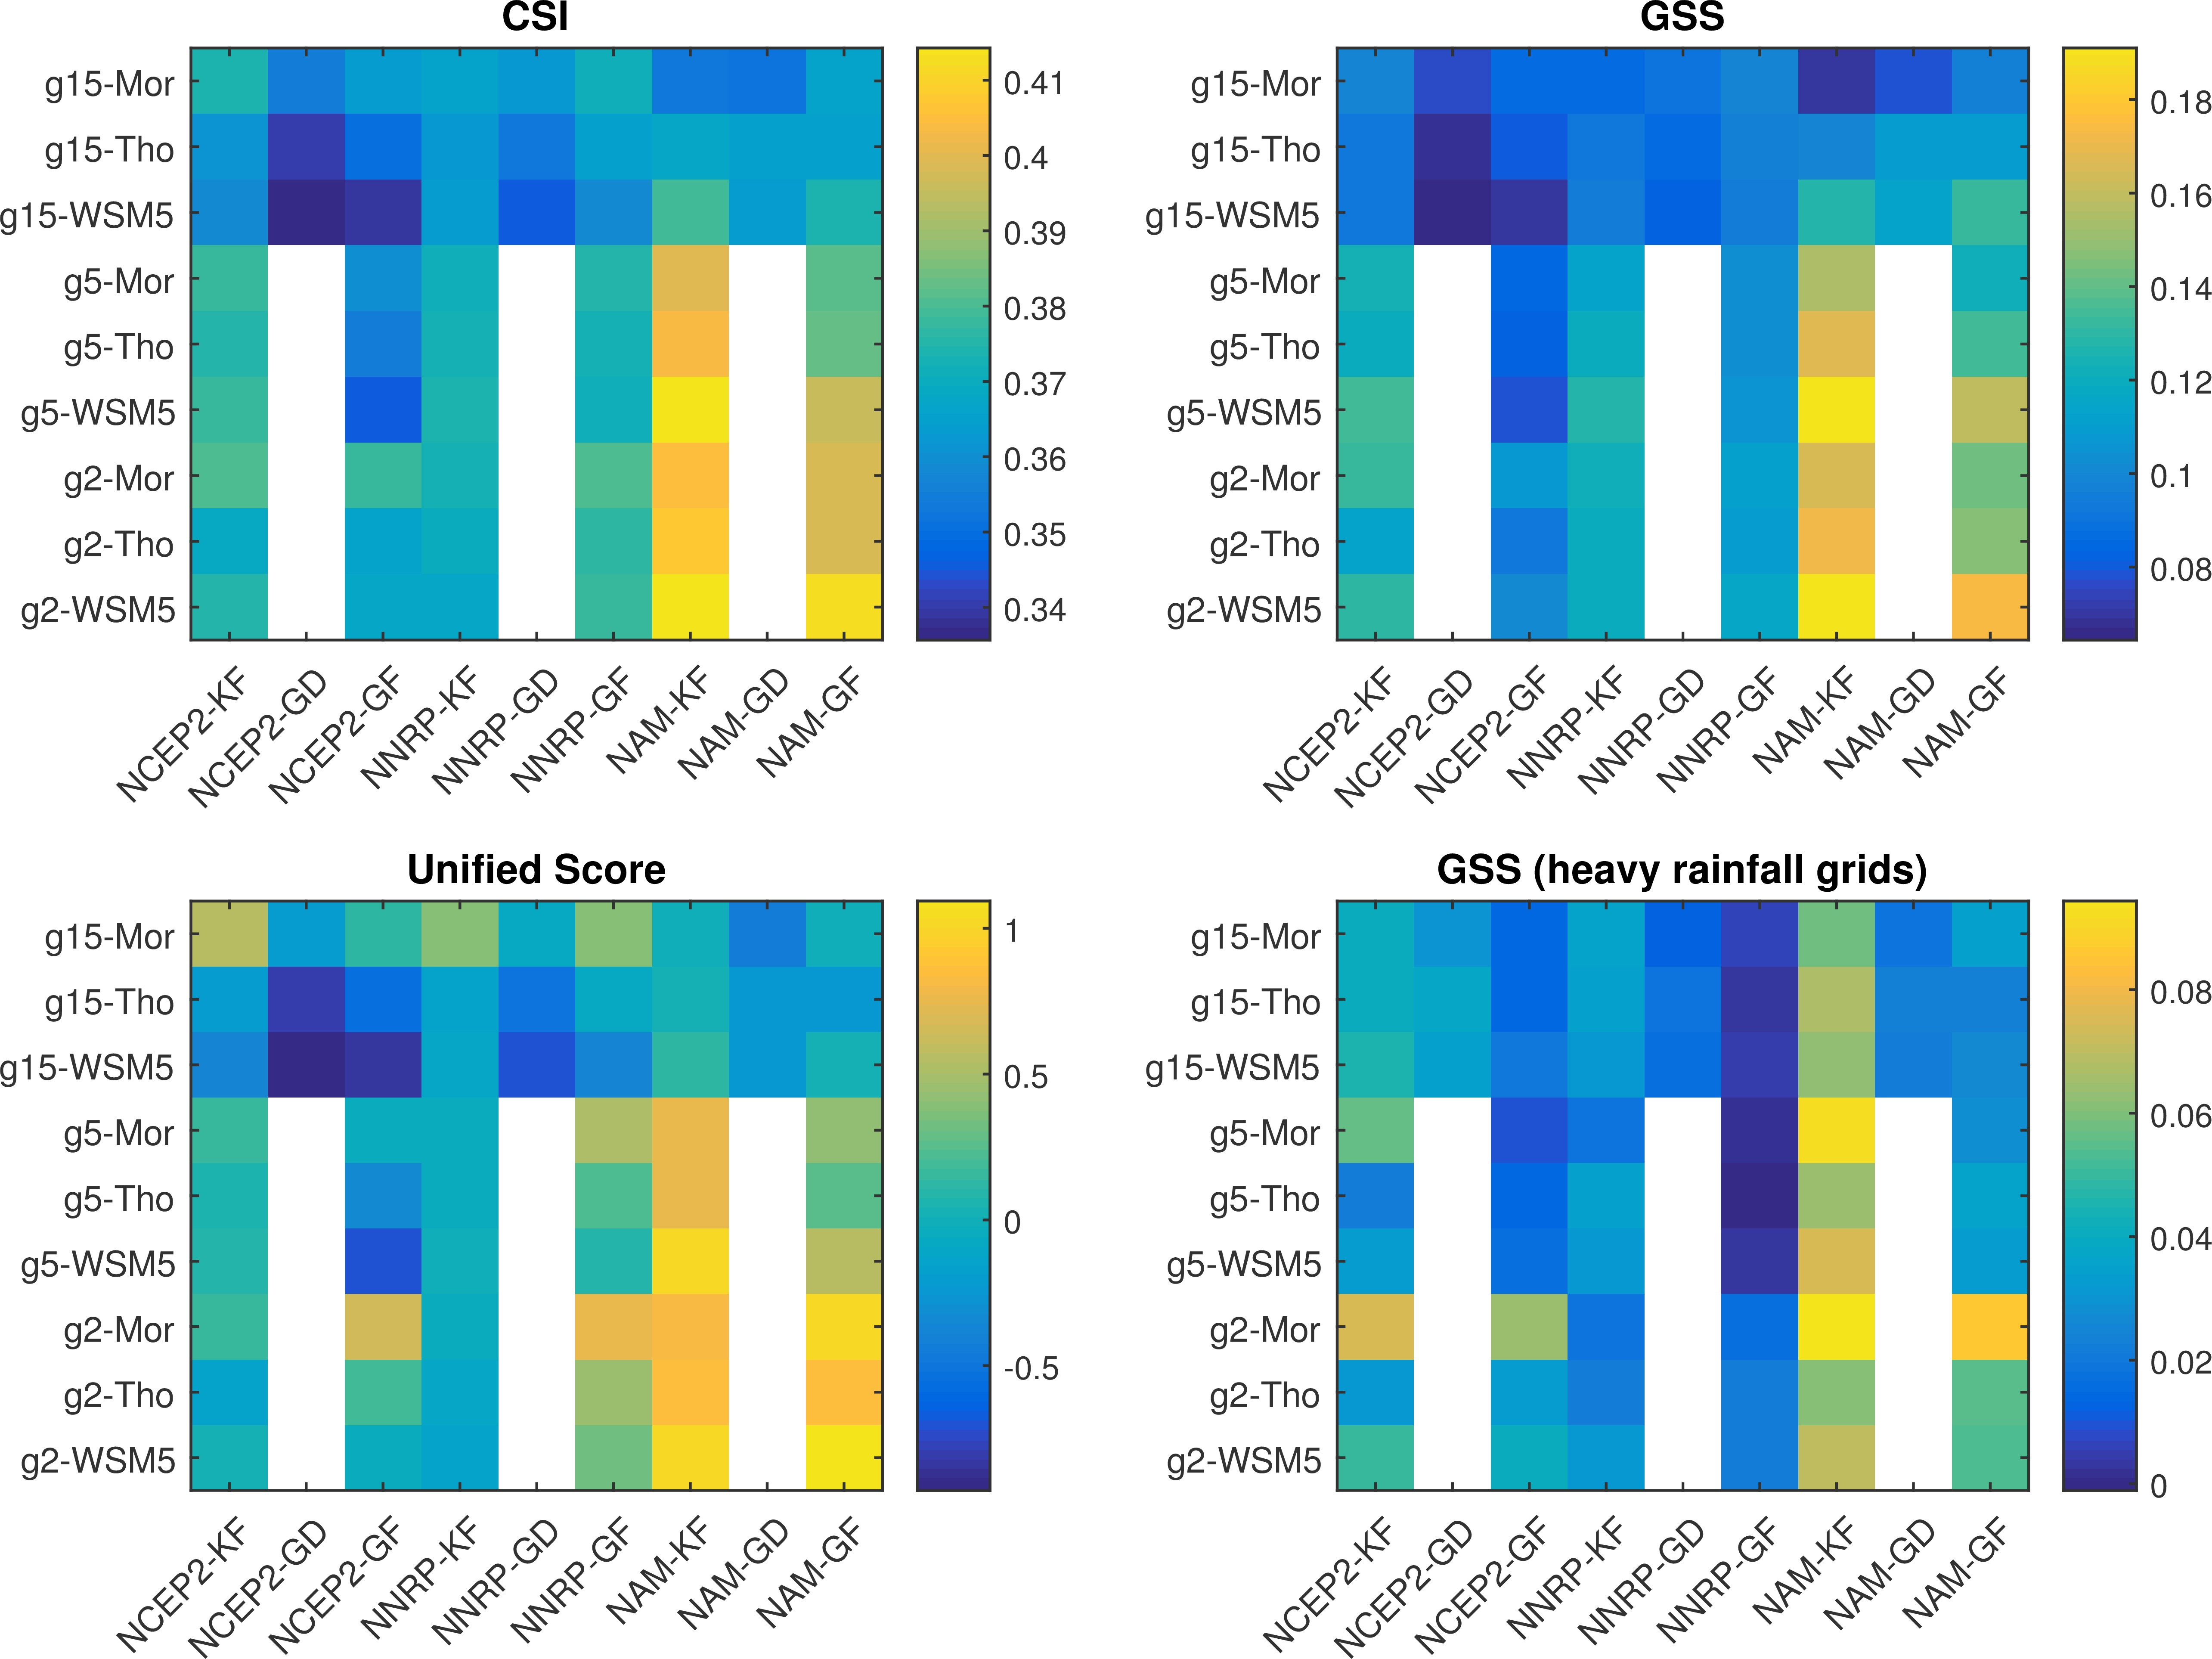
\includegraphics[width=\linewidth]{pics/ch2/fig6.jpg}
  \caption{Evaluation of WRF reconstructions involving multiple aspects of rainfall simulation quality. Panel (a) shows $CSI$, (b) shows $GSS$, (c) shows unified score, (d) shows $GSS$ scores for the rain center.}
  \label{fig:2-6}
\end{figure}

As shown in the figures above, different metrics usually yield differing recommendation. They are helpful for specific purposes, but a better metric would be desired to simultaneously evaluate multiple aspects of the modeling framework. For this purpose, the unified scores ($US$, see equation \ref{eq:2-2}) were calculated and shown in panel \ref{fig:2-6}(c). At coarser grid (15km), the Morrison microphysics scheme provides the best results. With the NCEP2 IC/BC, the KF scheme yields the highest scores in the g15 domain setup (Figure \ref{fig:2-2}a) group. As the model is run in the finer grids, the NCEP2 results produce lower scores, and even negative sometimes. At the finer grids (5km and 2km), however, NAM yields the best detail estimates of rainfall. NNRP gives the worst results in both coarse and fine grids, and the scores degrade further in the finer grids. With NAM providing IC/BC, the 2km simulations are more skillful than the 5km simulations and less sensitive to the parameterizations used, though the extra improvement is marginal. It is also noted that GF cumulus scheme produces best US score in g5 and g2 domain setup. This implies the GF scheme is scale aware, and it does not double count the deep convection along with rainfall that is resolved by the microphysics process.

For extreme events, it is sometimes more useful to analyze the area with heavy rainfall, as they tend to result in heaviest human and economic losses. NOAA’s definition of heavy storm is those events with hourly rain rate larger than 7.6mm. Using this threshold to filter out non-heavy rainfall area, we can evaluate the model performance over the heavy rain area. Panel \ref{fig:2-6}(d) shows the $GSS$ for the Nashville 2010 event with only heavy ($>$7.6mm/hour) rainfall cells/time-steps are treated as rainy cells.

Unlike panel \ref{fig:2-6}(b), the KF cumulus scheme tends to work best in the heavy rain area. It is obvious that KF cumulus scheme is a winning option at various scales. At coarser resolution, WSM-5 microphysics scheme tends to work better, while Morrison is dominantly better at finer resolutions. The best modeling frameworks recommended by general $GSS$ scores (panel \ref{fig:2-6}b) are quite different from those highlighted by the heavy rain area $GSS$ scores, thus it is necessary to identify the specific objectives of the modeling framework, and choose the corresponding evaluation metrics.

In the applications where storm magnitude is important (e.g. when used as input to hydrological or hydraulic models), it is necessary to quantify the simulated rainfall in both spatial extent and amount. Here the simulated 48-hour rainfall maps are compared to Stage IV and Livneh data under Nash-Sutcliffe coefficient. The results are shown in Table \ref{table:2-5}, where the values in parentheses are the results between modeled data and Livneh reference. The higher the Nash-Sutcliffe coefficient is, the better the model predicts the rainfall pattern. When compared to Stage IV data, Morrison microphysics and KF cumulus schemes outperform others in both coarser and finer grids. The same is held when they are compared against Livneh reference, suggesting that their superiority is independent from the choice of reference. In terms of IC/BC, NAM produced best results, followed by simulations with NCEP2 data.

\begin{table}[htbp]
	\centering
	\caption{Nash-Sutcliffe metric between simulated and Stage IV and Livneh reference rainfall map in the Nashville 2010 storm event}
	\begin{threeparttable}
		\begin{tabular}{cccccccccc}
			\hline
			\multirow{2}{*}{MP} & \multicolumn{3}{c}{NCEP2} & \multicolumn{3}{c}{NNRP} & \multicolumn{3}{c}{NAM}\\
			\cline{2-10}
			& KF & GD & GF & KF & GD & GF & KF & GD & GF\\
			\hline
			\multicolumn{10}{l}{15-km grids}\\
			Morrison & 0.09 & 0.05 & -0.03 & -0.03 & 0.04 & -0.1 & 0.34 & 0.17 & 0.16\\
			& (-0.20) & (-0.04) & (-0.09) & (-0.43) & (-0.06) & (-0.24) & (-0.02) & (-0.08) & -0.01\\
			Thompson & 0.08 & 0.09 & 0 & -0.05 & 0.06 & -0.1 & 0.36 & 0.21 & 0.21\\
			& (-0.28) & (-0.01) & (-0.05) & (-0.48) & (-0.10) & (-0.28) & 0 & (-0.01) & (-0.01)\\
			WSM-5 & 0.09 & 0.08 & 0.01 & -0.03 & 0.07 & -0.11 & 0.33 & 0.18 & 0.12\\
			& (-0.18) & (-0.09) & (-0.11) & (-0.48) & (-0.09) & (-0.31) & (-0.01) & (-0.02) & (-0.01)\\
			\hline
			\multicolumn{10}{l}{5-km grids}\\
			Morrison & 0.17 & - & -0.09 & -0.02 & - & -0.08 & 0.59 & - & 0.21\\
			& (-0.16) & - & (-0.46) & (-0.38) & - & (-0.29) & -0.43 & - & -0.01\\
			Thompson & 0 & - & -0.04 & -0.01 & - & -0.07 & 0.48 & - & 0.22\\
			& (-0.69) & - & (-0.37) & (-0.46) & - & (-0.33) & -0.18 & - & -0.03\\
			WSM-5 & -0.02 & - & -0.05 & 0.01 & - & -0.06 & 0.48 & - & 0.26\\
			& (-0.59) & - & (-0.51) & (-0.52) & - & (-0.34) & -0.15 & - & -0.04\\
			\hline
			\multicolumn{10}{l}{2-km grids}\\
			Morrison & 0.34 & - & 0.24 & -0.06 & - & -0.06 & 0.58 & - & 0.47\\
			& -0.09 & - & -0.07 & (-0.48) & - & (-0.48) & -0.3 & - & -0.15\\
			Thompson & 0.2 & - & 0.07 & -0.06 & - & -0.04 & 0.47 & - & 0.38\\
			& (-0.25) & - & (-0.46) & (-0.56) & - & (-0.44) & -0.11 & - & (-0.05)\\
			WSM-5 & 0.19 & - & 0.13 & 0 & - & -0.01 & 0.49 & - & 0.36\\
			& (-0.41) & - & (-0.46) & (-0.62) & - & (-0.51) & (-0.01) & - & (-0.20)\\
			\hline
		\end{tabular}
		\begin{tablenotes}
			\small
			\item Numbers in parentheses are with Livneh reference. Stage IV 48-hour total precipitation map is used to evaluate the simulated 48-hour total precipitation. Livneh gridded daily precipitation data on May 1, 2010 is used to evaluate the simulated total precipitation on this day.
		\end{tablenotes}
	\end{threeparttable}
	\label{table:2-5}
\end{table}

To check the statistics of simulated rainfall intensity, we can plot the hourly rainfall intensities as histograms in Figure \ref{fig:2-7}. In these panels, the x-axis shows the hourly rainfall intensity, the y-axis shows the total count of such hourly rainfall intensities across the evaluation area in the 48-hour duration. Each panel in the figure shows a combination of IC/BC, microphysics and cumulus schemes. The black lines are the histograms from Stage IV data, the blues lines are those using g15 grids, red lines are those using g5 grids, green lines are from g2 grids. The biggest difference comes from grid size, where g15 results are often biased away from observation. In most cases, g5 results are closer to the observation, and the improvement from g5 to g2 is not significant. This confirms that g5 is a balance between accuracy and computing burden. Again, Morrison microphysics and KF cumulus schemes produced better results here.

\begin{sidewaysfigure}[htbp]
  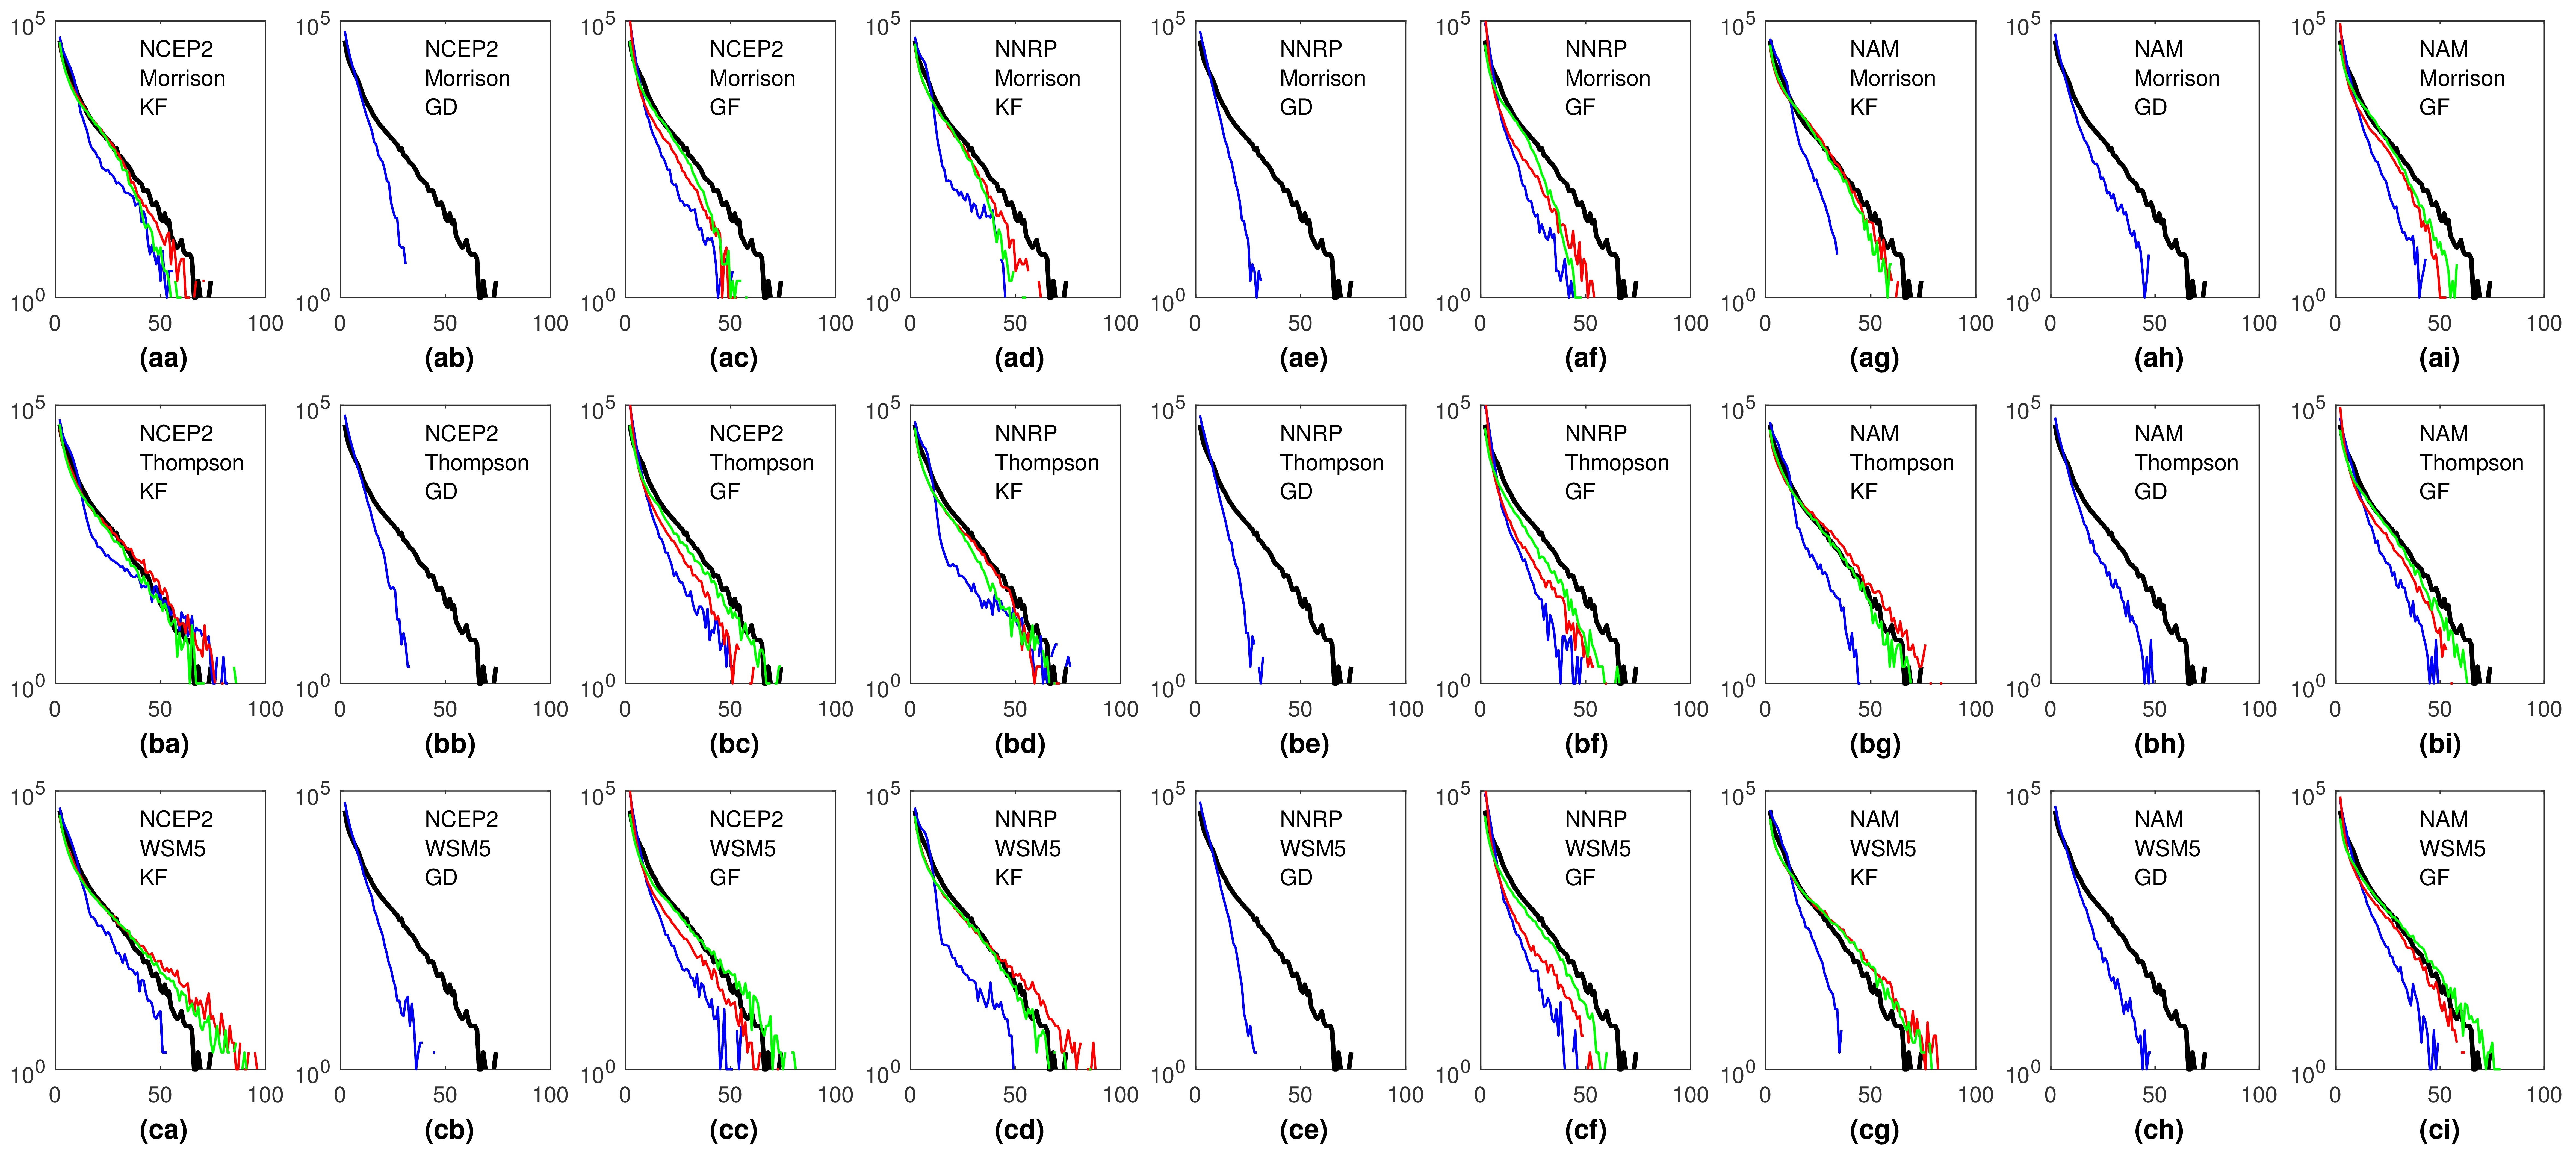
\includegraphics[width=\linewidth]{pics/ch2/fig7.jpg}
  \caption{Evaluation of hourly rainfall intensity histogram simulated by WRF.}
  \label{fig:2-7}
\end{sidewaysfigure}

Our evaluation suggests that different demands are best met with different model options for extreme storm simulation. These options have their own strengths and weaknesses. However, collectively they can be used to generate a multi-physics ensemble forecast, which is useful for providing an ``envelope" at a certain confidence level for an engineering application. For example, a range of possible PMP estimates can be much more useful for risk management than a single deterministic value. Our results show that the width of the envelope is largely determined by uncertainty in the IC/BCs, followed by sensitivity to grid resolution. The use of the scale-aware GF scheme tends to reduce model sensitivity to resolution as intended and consistently yields the high unified scores regardless of the microphysics parameterizations used. These results demonstrate the possibilities of capturing the full range of the envelope using fewer but carefully tested configurations of the end members for design PMP estimates.

In summary, NAM is better for the finer grids simulation, while NCEP2 is also a good choice at coarser grids for extreme storms. At finer grids, Morrison or WSM-5 is often a winning option. At coarse grid scale, the results from different microphysics and cumulus schemes are mixed. Combinations that better resolve the spatial-temporal structure of the storm are: g15-NAM-Morrison-KF, g5-NAM-Morrison-KF, g15-NCEP2-Thompson-GF, g5-NAM-WSM5 (with KF or GF cumulus parameterization scheme). The improvement from g5-NAM-WSM5 to g2-NAM-WSM5 is insignificant (e.g. CSI changed from 0.40 to 0.41), so given the larger computing requirements, the g2 option is not recommended here. For general purpose, we recommend NAM-Morrison-KF as a starting choice. With enough computing capacity, g5 grid is recommended, but g15 is also acceptable when running with this configuration.

For the Nashville 2010 storm reconstruction, our recommendation emerging from the application of the framework differs from previous studies. For example, \textit{Mahoney} [2013] recommended the 4km-1.3km nested grids, the NAM forecast IC/BC with the new Thompson microphysics and no cumulus schemes. The maximum 48-hour total rainfall captured by \textit{Mahoney} [2013] was 260mm, while in our study, it is 239 mm from the 1.6km grid. However, the WSM-5 scheme was not tested by \textit{Mahoney} [2013]. In our study, the 300mm 48-hour total rainfall isohyet was captured by using the WSM-5 microphysics scheme. Although these estimates are smaller than the maximum 48-hour total rainfall from the Stage IV reference precipitation data (330mm), the use of WSM-5 represents an advance in capturing the high-precipitation area.

In our study, we have included the 4 major factors that affect the atmospheric model performance. However, there are still some other factors that can be fine-tuned as needed, such as land surface process, planetary boundary scheme, land use condition. Following the same methodology outlined in this study, these factors can be added into this evaluation framework to achieve even better simulation quality, if desired by the engineering community.

\section{Validation of optimal model configuration}

We proved that our recommended model configuration is independent from reference choice. The representativeness of this finding for other storms remains a question. Therefore, we applied the optimal WRF configuration to other two storm events, one is the 1997 January 1-3 storm in the American River watershed, California (denoted as ``1997-CA" event); the other is the 1980 December 24-26 storm in the Pacific Northwest region (``1980-PNW" event). Due to the data availability, these two events are reconstructed using the NCEP2 IC/BC.

The 1997-CA event happened in northern California, and caused a severe flood at Sacramento in the following days. The observed maximum 24-hour precipitation was 284mm, which made it one of the greatest storms in this area. The 1980-PNW event happened in the Washington and Oregon, and the observed maximum 24-hour precipitation was 234mm. This storm is one of the big storms used in the HMR for PMP in the Pacific Northwest region (HMR57). The spatial domain of WRF simulations are illustrated in figure \ref{fig:2-S1}.

\begin{figure}[htbp]
  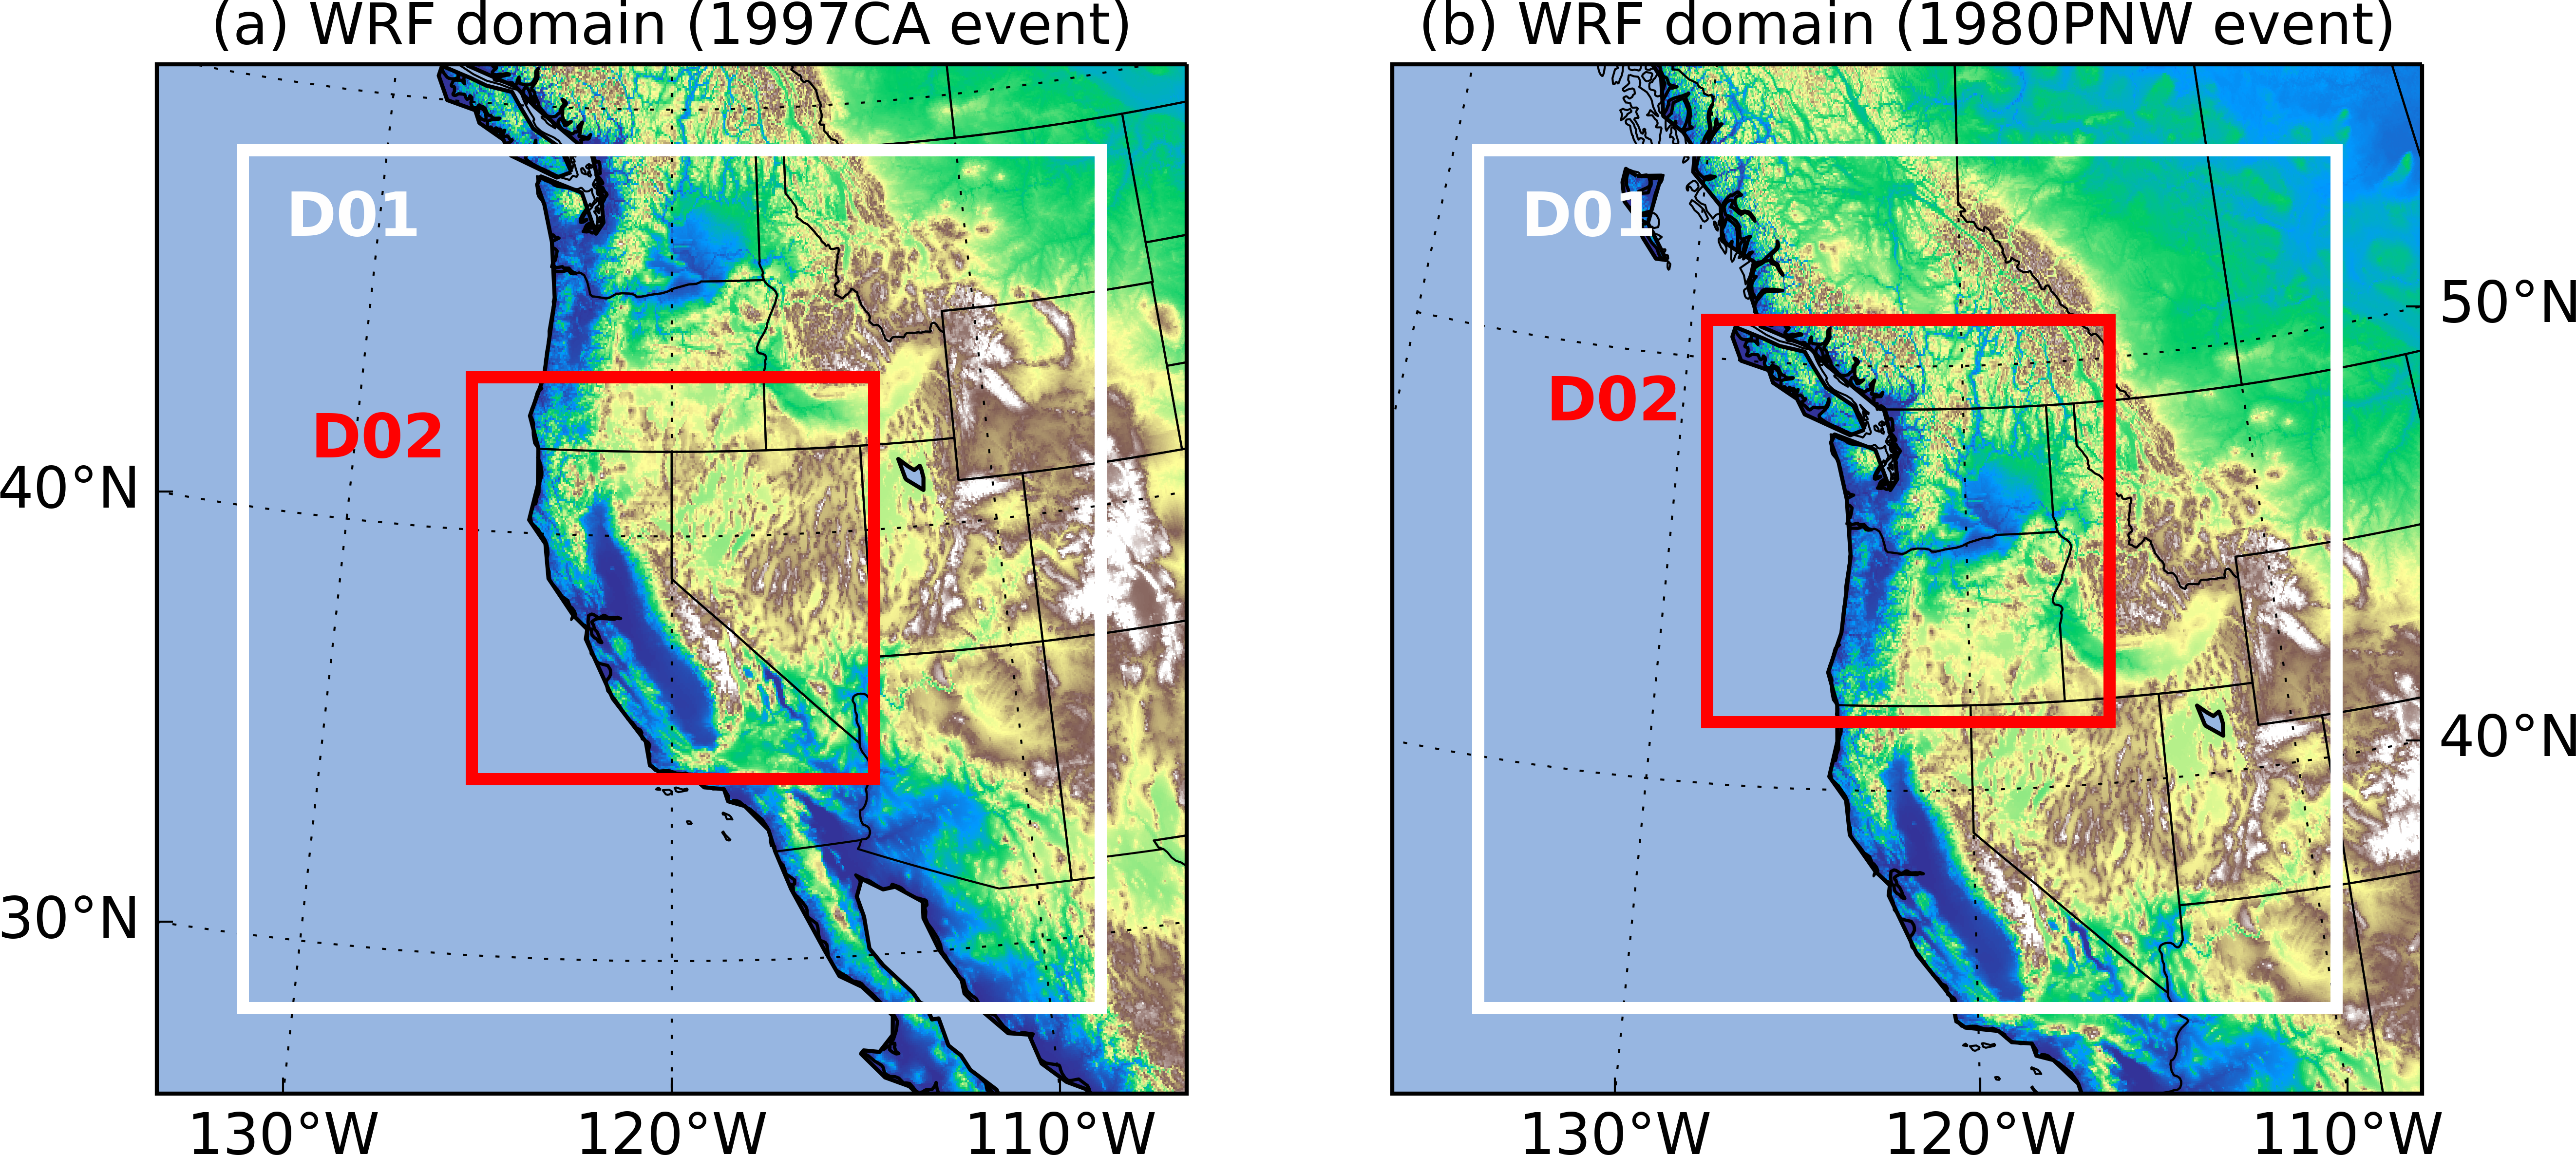
\includegraphics[width=\linewidth]{pics/ch2/figS_2events.png}
  \caption{Spatial domain in modeling framework of 1997-CA event and 1980-PNW event. Panel (a) is the 1997-CA simulation; (b) is the 1980-PNW simulation.}
  \label{fig:2-S1}
\end{figure}

We reconstructed these storm events using the optimal model configuration (15km-5km nested grids, Morrison microphysics and KF cumulus schemes) that was obtained through the Nashville 2010 study. The simulated 3-day total rainfall of these two events, plus the simulated 1-day rainfall of Nashville 2010 event, are shown in Figure \ref{fig:2-8}. Panels \ref{fig:2-8}(a) and \ref{fig:2-8}(d) show the model reconstructed 3-day precipitation, and panels \ref{fig:2-8}(b) and \ref{fig:2-8}(e) show the Livneh reference. The third column shows the different as WRF-Livneh. It shows that this model configuration depicts the heavy rainy area in both spatial extent and magnitude: In the 1997-CA simulation, the model captures the storm center along the Sierra Nevada; In the 1980-PNW simulation, it captures the heavy rainy band along the coast.

\begin{figure}[htbp]
  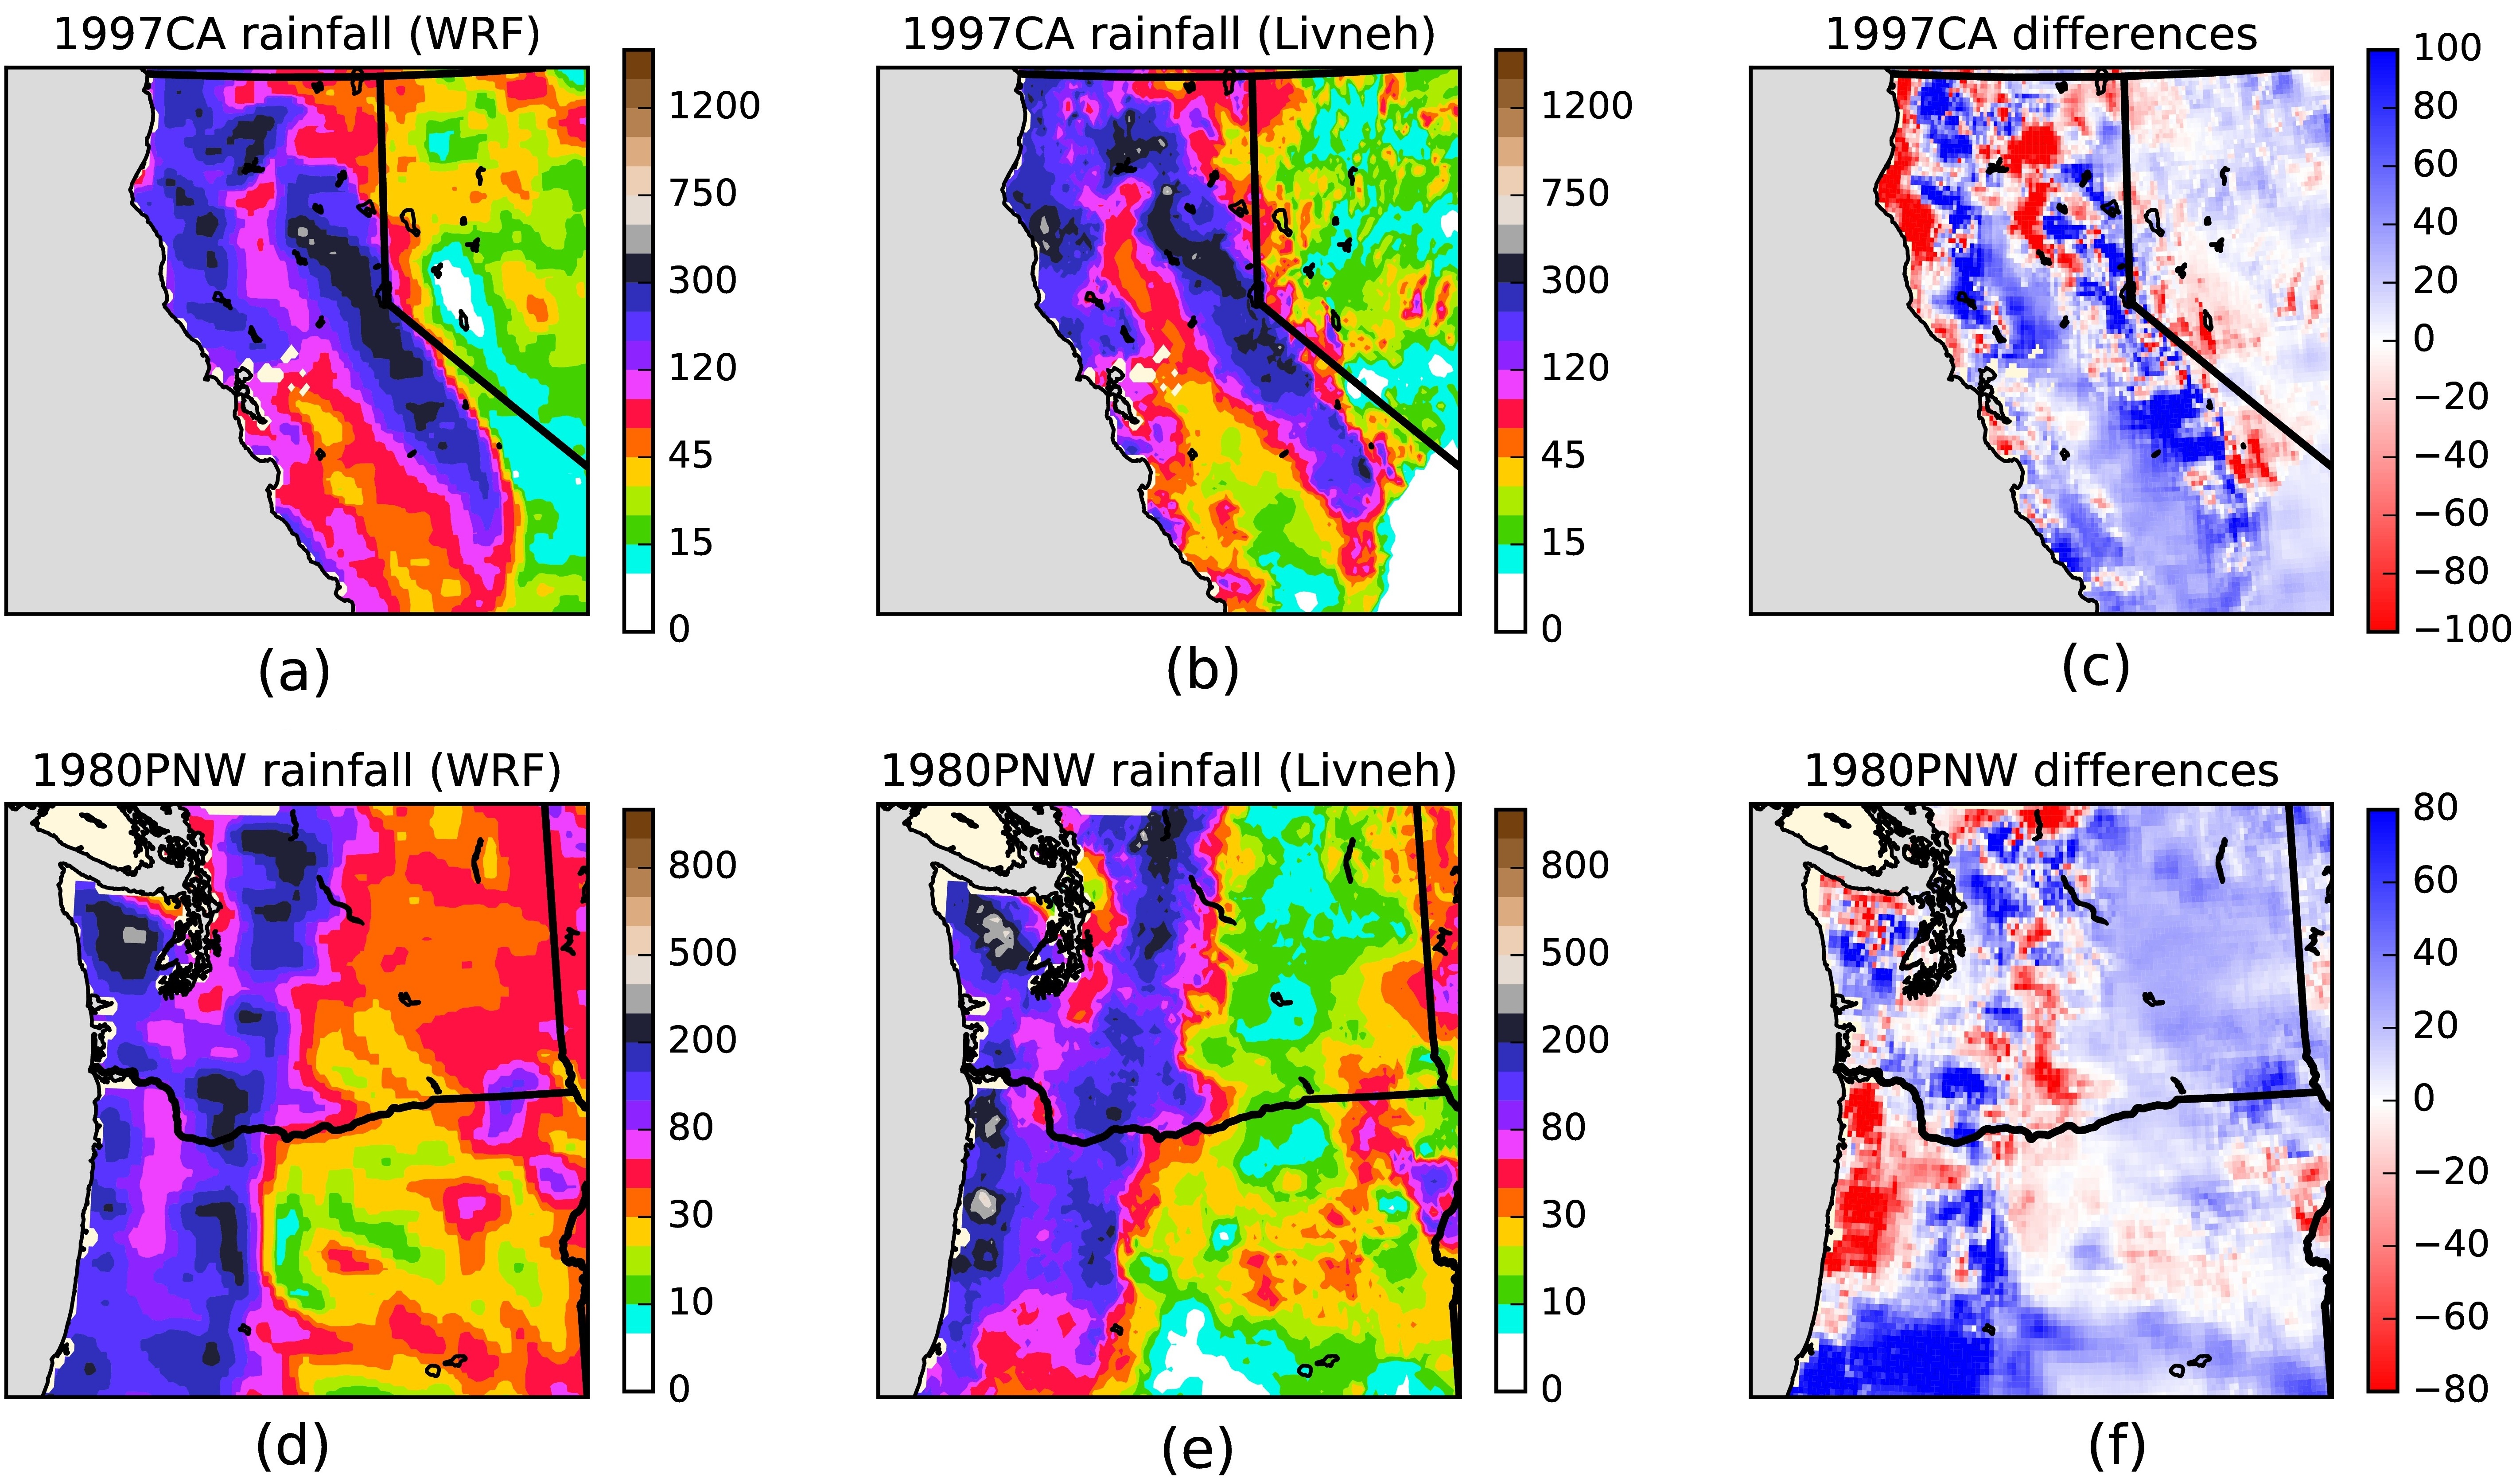
\includegraphics[width=\linewidth]{pics/ch2/fig8.jpg}
  \caption{Evaluation of 1997-CA and 1980-PNW storms using optimal WRF configuration. The left columns are the WRF reconstructions of the two events; the middle columns are the observed rainfall; the right columns are the difference between WRF reconstruction and observation.}
  \label{fig:2-8}
\end{figure}

To quantity the performance of these reconstructions, we also tested all the 9 model configurations in 15km grids, and 6 configurations in 15km-5km grids. The evaluation of Nash-Sutcliffe coefficient on the simulated maximum 3-day rainfall is shown in Table \ref{table:2-6}. In the 1997-CA simulations, this optimal configuration (based on Nashville 2010 storm) produced the best result. In the 1980-PNW simulations, the performance of this optimal model configuration is within the top 3 among all the experiments. This confirms the capability of our optimal model configuration in reconstructing other severe storms, and this is independent of the choice of reference data.

\begin{table}[htbp]
	\centering
	\caption{Nash-Sutcliffe metric between simulated and Livneh reference 3-day cumulative rainfall map in the 1997CA and 1980PNW storm events}
	\begin{threeparttable}
		\begin{tabular}{ccccccc}
			\hline
			\multirow{2}{*}{MP} & \multicolumn{3}{c}{1997-CA} & \multicolumn{3}{c}{1980-PNW} \\
			\cline{2-7}
			& KF & GD & GF & KD & GD & GF\\
			\hline
			\multicolumn{7}{c}{15-km grids}\\
			Morrison & \textbf{0.69} & 0.67 & \textbf{0.69} & \textbf{0.53} & \textbf{0.54} & \textbf{0.52}\\
			Thompson & 0.61 & 0.59 & 0.62 & 0.50 & 0.50 & 0.50\\
			WSM-5 & 0.59 & 0.57 & 0.63 & 0.41 & 0.41 & 0.40\\
			\hline
			\multicolumn{7}{c}{5-km grids}\\
			Morrison & \textbf{0.64} & - & \textbf{0.68} & 0.49 & - & 0.49\\
			Thompson & 0.57 & - & 0.63 & 0.46 & - & 0.47\\
			WSM-5 & 0.52 & - & 0.61 & 0.31 & - & 0.33\\
			\hline
			\end{tabular}
		\begin{tablenotes}
			\small
			\item Livneh gridded precipitation data ia used as reference.
		\end{tablenotes}
	\end{threeparttable}
	\label{table:2-6}
\end{table}

\section{Conclusions}

In this study, we investigated an approach to establish an optimal WRF-based framework for extreme storm event simulation. Our goal was to introduce a more physically-based method to the engineering design and analyses community currently engaged in large water management infrastructure issues of today and tomorrow. This framework takes into consideration the uncertainties coming from various IC/BC data sources, grid resolutions, cloud microphysics and cumulus parameterization schemes. These are the major contributors to the final model performance.

In the demonstration, we established a WRF-based modeling framework for extreme storm events in the CONUS region based on the Nashville 2010 storm, and validated it using two other storms in California and the Pacific Northwest. Based on the engineering intent, the best model configuration can be different. For general purpose, we recommend the WRF model configured as: 15km or nested 15km-5km grids, NCEP2 or NAM boundary condition, Morrison microphysics scheme with Kain-Fritsch cumulus scheme. This configuration is either the optimal configuration, or a starting point that leads to quick converge to the final optimal configuration.

As future studies, we hope to complete application and validation of the optimal WRF modeling framework for a large number of storms that were maximized for PMP estimation in HMR reports. As the use of atmospheric numerical models for engineering infrastructure analyses is gaining popularity among the infrastructure community, future studies should focus on improving current design and practice among engineers. Some examples are: 1) exploration of physics-based probable maximum flood (PMF; the flood due to PMP); 2) impact of land use/land cover change and global warming on PMP and PMF during extreme storms; 3) improving streamflow forecast and thus improving reservoir/dam operation during extreme storm events; 4) multi-physics ensemble-based analyses of numerical model output for risk management.


